\section{Latency Measurements}\label{sec-measure}


An important first step to taming in/outbound latencies is to
understand the various factors that affect them 
within the SDN switch. We conduct a variety of measurements aimed at
carefully isolating these factors. To draw general observation, we use
2 commercial switch platforms (Table~\ref{switch_para}).
To ensure that we are experimenting in the optimal regimes for the different
switches we take into account switch specifics such as maximum flow table sizes
as well as support for priority in rule set up. 
%We also make the distinction on the types of rule tables supported by the
%different switches.  
%1) Broadcom 956846K, 
%2) Intel FM6000 (model IZ1), 
%and 3) HP Procurve 8212zl.
%The specific details for each switch are shown in 
%\keqhe{Broadcom switch can only support proactive rule insertions while Intel
%and HP switch can support both proactive and reactive rule insertions.} 
\begin{table}
\centering
\small
\begin{tabular}{|l|l|l|l|l|}
\hline
Switch & CPU & RAM & \tabincell{c}{Flow \\Table Size} & Data Plane \\ \hline
\tabincell{c}{Broadcom \\956846K} & 1Ghz & 1GB & 896 & \tabincell{c}{14*10Gbps \\+ 4*40Gbps}\\ \hline
Intel FM6000 & 2Ghz & 2GB & 4096 & \tabincell{c}{40*10Gbps \\+ 4*40Gbps} \\ \hline
%\tabincell{c}{HP Procurve \\8212zl} & 666Mhz & 256MB & $\approx$1000 & Modularity \\ \hline
%\hline
\end{tabular}
\caption{Specific details of the switches}{\label{switch_para}}
\end{table}

%%\marina{We need a table with specific details of the switch - Switch type, Processor RAM, Data plane capacity, Max Flow table size, hardware and software tables, support for prioity, statistics gathering support}


\begin{figure}[!tb]
\centering
%%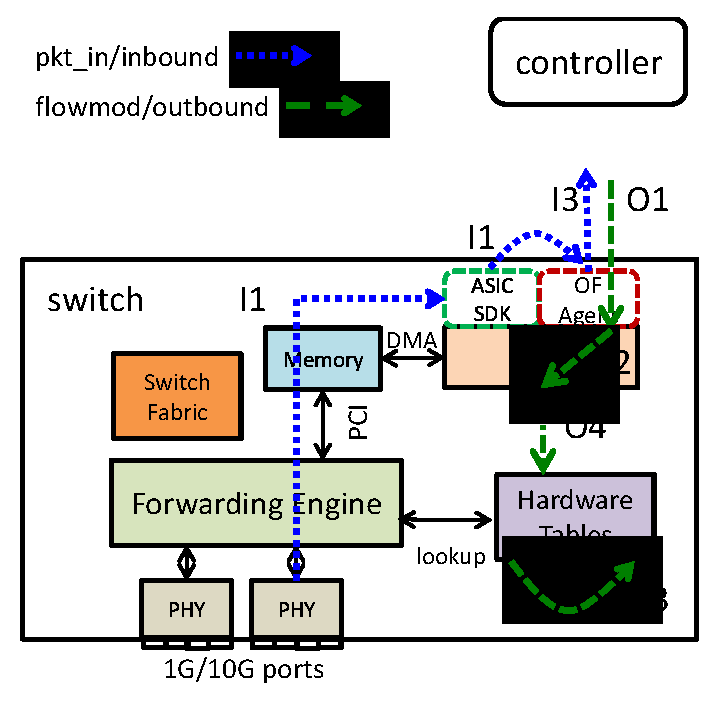
\epsfig{file=./figs/openflow_switch_illustrate.eps,width=0.4\textwidth} %%changed
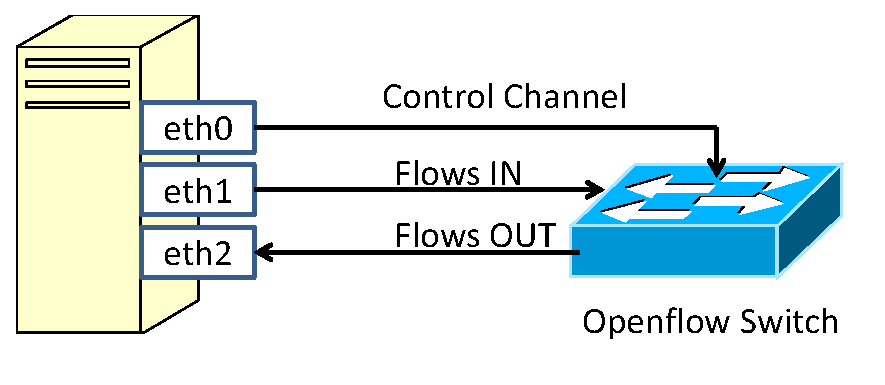
\includegraphics[width=2.2in]{figs/experiment_setup.eps}
\caption{Measurement experiment setup. }\label{experiment_setup} 
%\marina{add pox controller and pkt capture points on the fig}
\end{figure}

% and is similar to that used by~\cite{ucsdpaper}. 

\subsection{Measurement Methodology}
Our empirical setup is shown in
~\figref{experiment_setup}.
The host has one 1Gbps and two 10Gbps ports that are connected to the switch under test. 
The eth0 port is connected to the control port of the switch on one side and
a POX SDN controller running on the host is set to listen on this port. 
The ports eth1 and eth2 are connected to the data ports on the switch. 
%To ensure that the switch is not bypassed the eth1 and eth2 ports have different network name spaces. 
The propagation delay between the switch and the controller is
negligible (about 0.1 ms). The controller is used to send a set of
Openflow 1.0 \flowmod\ commands to the switch in burst mode. To
generate traffic for the 10Gbps NIC on the data plane, we use
pktgen~\cite{pktgen} in kernel space. Using this generator we are
able to generate traffic at 600-1000 Mbps.

Prior work notes that accurate execution of open flow commands on
commercial switches can only be accurately observed in the data
plane~\cite{oflops}. Thus, our experiments are crafted toward ensuring
that the impact of various factors on the latencies can be measured
directly from the data plane (at eth2 in \figref{experiment_setup}), except for
\packetin\ part of inbound latency. We use
\emph{libpcap} running on a high performance host to accurately time
stamp the different packet and rule processing events of each flow. We
first log the timestamps in memory and when the experimental run is
completed, the results are dumped to the disk and processed. We use
the time stamp of the first packet associated with a particular flow
as the finish time of the corresponding \flowmod\ command. Further
details that depend on the specific issues we measure are presented in
later sections.

%  Other details of the measurement methodology is
% customized to clearly delineate the inbound and outbound delay
% components and will be discussed in the relevant sections.

%%\marina{We need a table with specific details of the switch - Switch type, Processor RAM, Data plane capacity, Max Flow table size, hardware and software tables, support for prioity, statistics gathering support}

\subsection{Dissecting Inbound Delay}
\label{s:measure_inbound}

%%inbound delay on HP
\begin{figure}
% \subfloat[Flow rate = 100/s, concurrent with \flowmod\ and \packetout\ \label{fig:intel_inbound_test1}]
%   {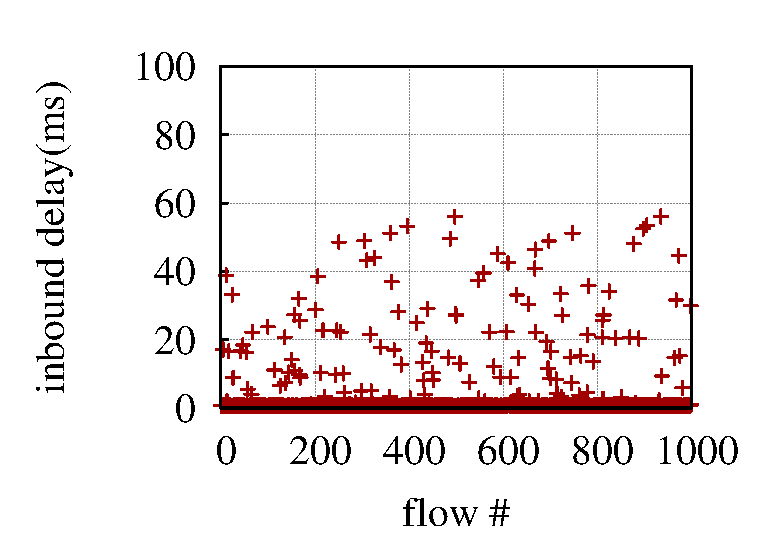
\includegraphics[width=.33\linewidth]{./figs/jan27_intel_inbound_with_pktout_flowmod_rate100.eps}}\hfill
%\subfloat[Flow rate = 200/s\label{fig:hp_inbound_test2}]
%  {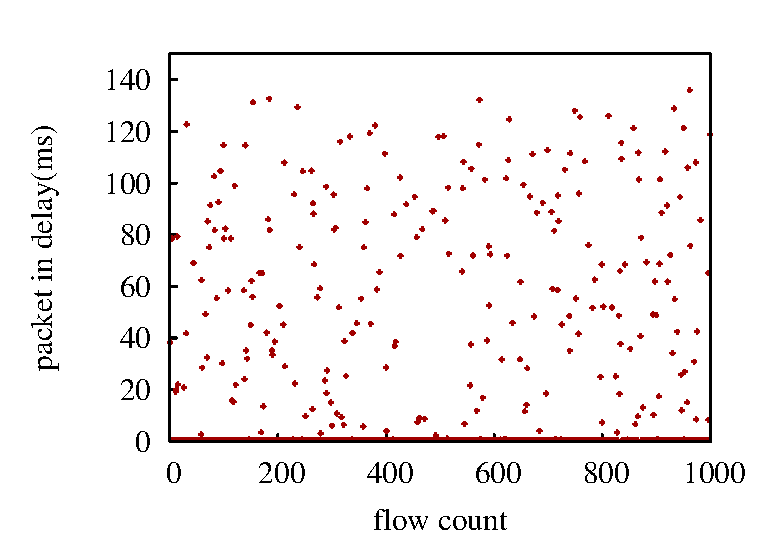
\includegraphics[width=.28\linewidth]{./figs/hp_inbound_delay_200.eps}}\hfill
\subfloat[with flow\_mod/pkt\_out \label{fig:intel_inbound_test3}]
  {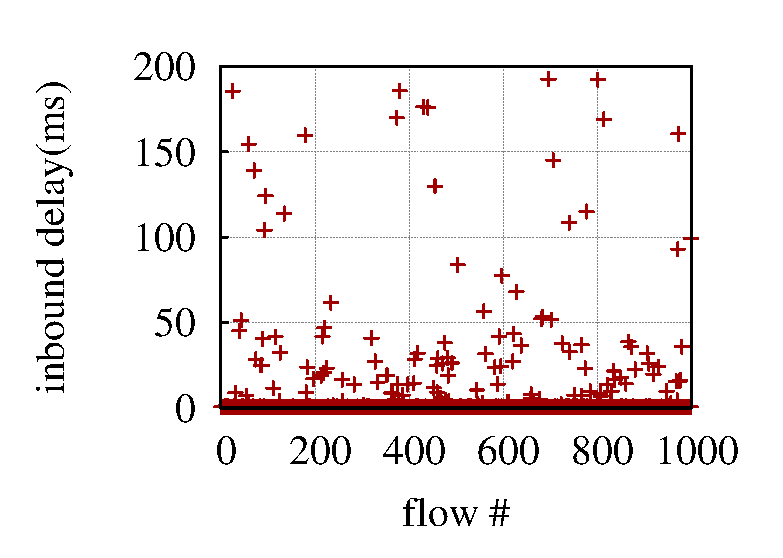
\includegraphics[width=.45\linewidth]{./figs/jan27_intel_inbound_with_pktout_flowmod_rate200.eps}}
\subfloat[w/o flow\_mod/pkt\_out \label{fig:intel_inbound_test3_wo}]
  {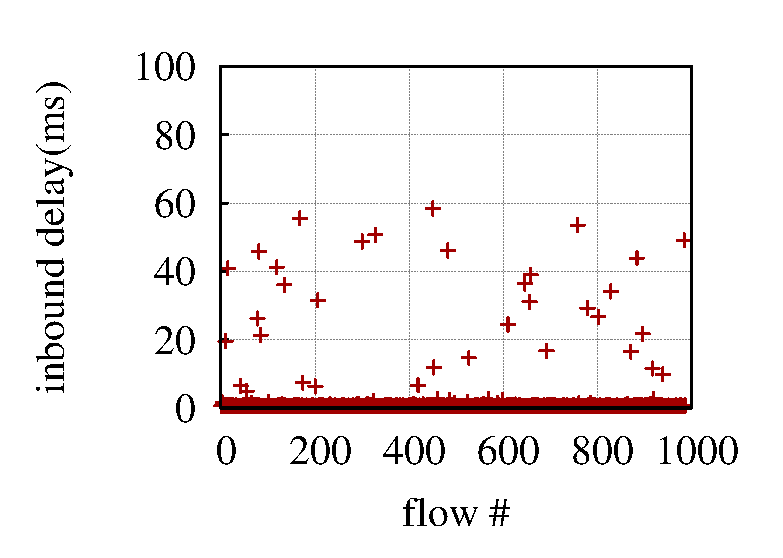
\includegraphics[width=.45\linewidth]{./figs/jan27_intel_inbound_wo_pktout_flowmod.eps}}
\caption{Inbound delay on Intel. Flow arrival rate = 200/s} 
%(a): with concurrent \flowmod\ and \packetout\ operations;
%  (b) without concurrent \flowmod\ and \packetout\ operations}
\label{fig:inbound-1}
\end{figure}

%\emph{Inbound delay:}
To capture inbound delay, we empty the table at the switch. We
generated traffic such that \packetin\ events are generated at a
certain rate (i.e., we create packets for new flows at a fixed
rate). To isolate the impact of \packetin\ processing from other
message processing, we perform two kinds of experiments.
In the first experiment, the \packetin\ will trigger corresponding
\flowmod\ and \packetout\ messages; the \flowmod\ messages insert
simple OpenFlow rules (differing just in destination IP).
%\aditya{Check previous sentence} 
In the second experiment, the \packetin\ message is dropped silently by the controller. 

We record the timestamp ($t_1$) when each packet is transmitted on the
measurement server's NIC. We also record the timestamp ($t_2$) when the server
receives \packetin\ message. The difference $t_2 - t_1$ is the inbound
delay.\footnote{This measurement technique differs from the approach
  used in \cite{ucsdpaper}, where the delay was captured from the
  switch to the POX controller which includes the overhead at the
  controller.}

%\marina{Where are the figures for the inbound delay. Explain how we isolate this
%  type of delay by dropping the pkt at the controller}. 

%%%%HP switch CPU  usage%%%%%%%%%

\begin{table}
\centering
\begin{scriptsize}
\begin{tabular}{cc}
\begin{tabular}{|c|c|c|}
\hline
\multicolumn{3}{|c|}{with flow mod/pkt out} \\ \hline
flow rate & 100/s  & 200/s  \\ \hline
cpu usage & 15.7\%    & 26.5\%   \\ \hline
\end{tabular}
&
\begin{tabular}{|c|c|c|}
\hline
\multicolumn{3}{|c|}{w/o flow mod/pkt out} \\ \hline
flow rate & 100/s   & 200/s \\ \hline
cpu usage & 9.8\%     & 14.4\%   \\ \hline
\end{tabular}
\end{tabular}
\caption{CPU usage on Intel switch}
\label{fig:inbound-cpu}
\end{scriptsize}
\end{table} 
%\li{is the following sentence correct?}
%When the controller receives \packetin\ message, the controller will drop it. As
%we keep sending packets, it will allow us to repeatedly measure inbound delay. 

Representative results for these two experiments are shown in
Figures~\ref{fig:inbound-1}(a) and (b), respectively, for the Intel switch; results
for the Broadcom switch are qualitatively similar.
For the first experiment (a), we see that the
inbound delay is quite variable with a mean of 8.33 ms and standard
deviation of 31.34; also, it increases with the \packetin\
rates (e.g., the mean is 3.32 ms for 100/s; not shown). For the second experiment (b) the inbound delay is
significantly small for most of the time. The only difference across
the two experiments is that in the former case, the switch CPU is processing
\flowmod\ and \packetout\ alongside generating \packetin\ messages. As such, we see significant CPU
utilization during this experiment (Table~\ref{fig:inbound-cpu}).
Thus, we conclude that inbound delay is mainly caused by switch CPU
and due to interference with \flowmod\ and \packetout\ processing.
 
\subsection{Dissecting Outbound Delay} 
\label{s:outbound_meas}

%We define the egress delay as the difference between the time when the switch
%issues the flow\_mod and/or packet\_out message and the time when the first
%packet of a particular flow is sent out by the switch. 
% We used the customized controller interfaces to control the \flowmod\ message
% generation. 
%by controlling the matching fields and priorities of the \flowmod\ messages. 

Before we perform the outbound delay measurements, first we install a single
default low priority rule which instructs the switch to drop all the traffic.
Then we install specially designed Openflow rules at the switch; while
they simply specify the destination IP address leaving other fields
wildcarded, they  may have different priorities. All 
instruct the switch to output traffic to the port which is connected  
to the measurement host on which we are monitoring.  

% By default, the table
% has only one rule that drops all packets~\footnote. 
%\li{Is the default rule has a lower
%  priority in the same priority experiment? Should we say this does not impact
%  our experiemental results? }

We examine outbound latencies for three different \flowmod\
operations in turn, namely, insertion, modification and deletion. We
examine the impact of key factors on these latencies, namely, table
occupancy and rule priority structure.

%\marina{give an example of what we mean increasing rule priority and decreasing
%  rule priority}. 
%Our egress delay measurements make a distinction between the
%flow\_mod and pkt\_out events.  
%By contrast previous measurement work \ref{maple, ucsdHiFi13} for egress delay, only
%captured the "packet out" delay. Thus our approach helps provide a more detailed
%analysis of the egress delay.  

% The priority of a rule indicates its position in the TCAM. Inserting a higher priority
% rule can displace many lower priority rules. To investigate how priority rule
% affects outbound delay. We perform a burst of $n$ \flowmod\ operations with the
% same, increasing, decreasing priority respectively. The \flowmod\ operations are
% insertion, modification and deletion. We also vary $n$. 

\subsubsection{Insertion Latency}
\label{s:meas_insert}

\begin{figure*}[!tb]
\centering
\subfloat[burst size 100, same priority\label{fig:bcm_burst_100_same_pri}]
  {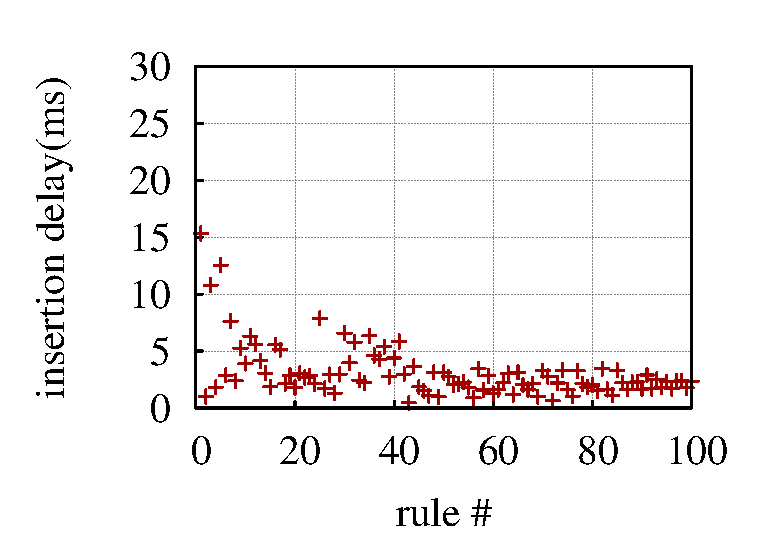
\includegraphics[width=.24\linewidth]{./figs/jan27_bcm_add_same_burst_100.eps}}\hfill
\subfloat[burst size 200, same priority\label{fig:bcm_burst_200_same_pri}]
  {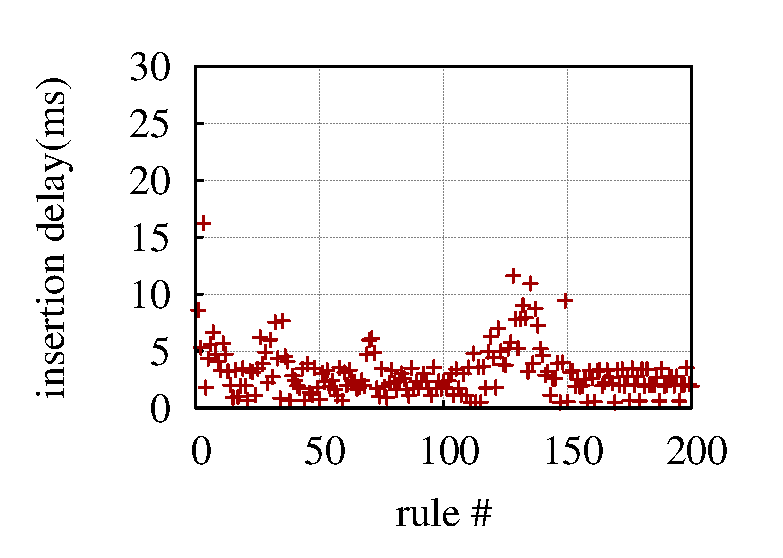
\includegraphics[width=.24\linewidth]{./figs/jan27_bcm_add_same_burst_200.eps}}\hfill
\subfloat[burst size 100, incr. priority\label{fig:bcm_burst_100_incr_pri}]
  {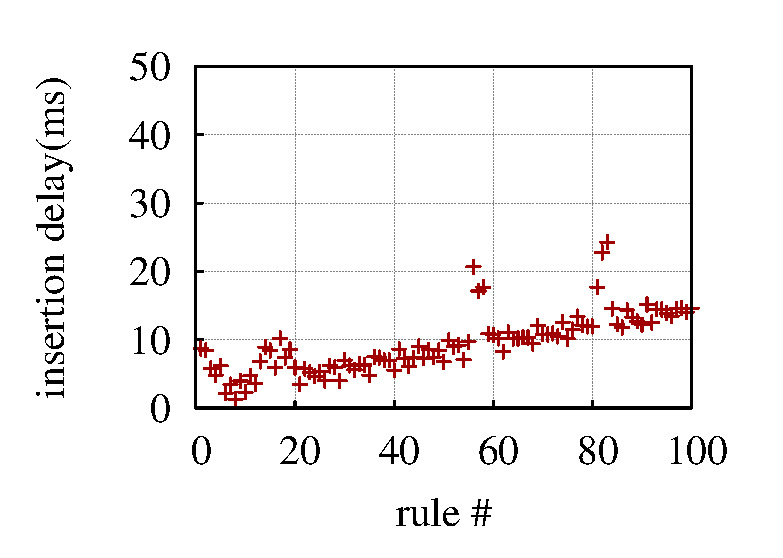
\includegraphics[width=.24\linewidth]{./figs/jan27_bcm_add_incr_burst_100.eps}}\hfill
\subfloat[burst size 200, incr. priority\label{fig:bcm_burst_200_incr_pri}]
  {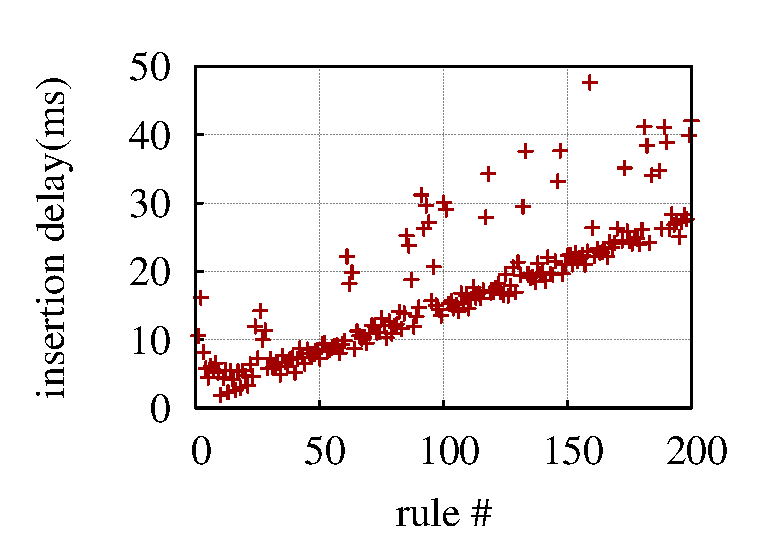
\includegraphics[width=.24\linewidth]{./figs/jan27_bcm_add_incr_burst_200.eps}}
\topcompactcaption{{\bf \BroadcomOne} priority per-rule {\bf insert} latency}
\label{fig:priority-broadcom-insert}
\end{figure*}


We first examine how different rule workloads impact insertion latency. We
insert a burst of $B$ rules: $r_1,\cdots,r_B$. Let $T(r_i)$ be the time we
observe the first packet matching $r_i$ emerging from the output port
specified in the rule. We define per-rule insertion latency as $T(r_i)-T(r_{i-1})$.  

%We conduct a variety of tests to examine how different patterns of
%rule workloads impact insertion latency. In almost all experiments, we
%install a burst of rules. Let us denote these rules
%in a sequence as $r_1, r_2,\cdots,r_i,\cdots, r_B$. Denote $T(r_i)$ as the time we
%observe the first packet matching $r_i$ emerging from the intended port of the rule
%action. We define insertion latency as $T(r_i)-T(r_i-1)$.  

\minisection{Rule Complexity} 
To understand the impact of rule complexity (i.e., the number of header 
fields specified in a rule), we install bursts of rules that specify either
2, 8, or 12 fields. In particular, we specify destination IP and EtherType
(others wilcarded) in the 2-field case; input port, EtherType, source and
destination IPs, ToS, protocol, and source and destination ports in the
8-field case; and all supported header fields in the 12-field (exact match)
case. We use a burst size of 100 and all rules have the same priority.

%To understand the impact of rule complexity (i.e., the number and type of
%matching fields specified in a rule), we conduct three different
%experiments with a fixed burst size ($B$ = 100) and priority but the rules
%having different matching fields. In the first experiment, all the rules in a
%burst only have only 2 match fields (others wildcarded), in the second
%experiment all the rules have 8 match fields (others wildcarded), and in the
%third experiment the rules have all the 12 match fields set (exact match).
%For the 2-match field experiment, we specified the destination IP and
%EtherType as the matching fields and for the 8-match field experiment we
%specified all the matching fields except source mac, destination mac, vlan id
%and vlan priority.  

We find that rule complexity {\em does not} impact insertion latency. The
mean per-rule insertion delay for 2-field, 8-field, and exact
match cases is 3.31ms, 3.44ms, and 3.26ms, respectively, for \BroadcomOne.
Similarly, the mean per-rule insertion delay for \Intel, \IBM, and
\BroadcomThree is $\approx$ 1 ms irrespective of the number of fields. 
All experiments that follow use rules with 2 fields.

%\emph{\BroadcomOne:} The mean per rule insertion delay is 3.31, 3.44 and 3.26 ms for 2-match field, 8-match field and exact match experiments respectively. This indicates that the insertion time does not vary with rule complexity on \BroadcomOne.

%\emph{\BroadcomThree:} 
%We observed that when a burst of rules is inserted, the \BroadcomThree firmware organizes the rules into batches. 
%Each batch has a size of about 50 rules and a single batch of rules is scheduled for insertion every 4 seconds. 
%This effect adds significant delay (4 seconds) between processing of two consecutive batches.
%This can be attributed to the inefficent firmware implementation which is still in its early stage of development. 
%We assume that the batching effect is due to unoptimized firmware and will be fixed in the near future. 
%Hence, we only consider the batch completion time when discussing insertion time on \BroadcomThree.  


%For 2-field, 8-field and exact match experiments the mean batch completion time 
 %(mean per rule insertion time) 
%is about 47 ms, 45 ms, 51 ms. This indicates that the %insertion time is not dependent on rule complexity on %\BroadcomThree neither. 

\minisection{Table occupancy} To understand the impact of table occupancy, we
insert a burst of $B$ rules into a switch that already has $S$ rules
installed. All $B+S$ rules have the same priority. We fix $B$ and
vary $S$, ensuring $B+S$ rules can be accommodated in each switch's hardware
table.

%\li{TODO: Keqiang, please add corresponding numbers in text for Broadcom and
%  Intel. } 

We find that flow table occupancy {\em
does not} impact insertion delay if all rules have the same priority.
Taking $B=400$ as an example, the mean per-rule insertion delay is 3.14ms, 
1.09ms, 1.12ms, and 1.11ms (standard deviation 2.14ms, 1.24ms, 1.53ms, and
        0.18ms) for \BroadcomOne, \BroadcomThree, \IBM
and \Intel, respectively, regardless of the value of $S$. 
%However, flow table occupany has an indirect impact through priority which
%we will cover next.  investigate in Section~\ref{sec:priority}. 

\minisection{Rule priority} To understand the effect of rule priority on the
insertion operations, we conducted three different experiments each covering
different patterns of priorities. In each, we insert a burst of $B$ rules
into an empty table ($S=0$); we vary $B$. In the {\em same priority}
experiment, all rules have the same priority. In the {\em increasing} and
{\em decreasing priority} experiments, each rule has a different priority and
the rules are inserted in increasing/decreasing priority order, respectively. 

\emph{\BroadcomOne, same priority.} 
%We experimented with several values of $B$. 
Representative results for $B=100$ and $B=200$ are shown in
\figsref{fig:bcm_burst_100_same_pri}{fig:bcm_burst_200_same_pri}, respectively. In both
cases, we see that the per-rule insertion delay is similar: with
medians of 3.12ms and 3.02ms, and standard deviations of 1.70ms and 2.60ms, 
for $B=100$ and $B=200$, respectively. 
% insert $B=100$ rules in the
% switch. As shown in Figure~\ref{fig:priority-broadcom-insert}-a, the per rule
% insertion delay among the 100 rules are similar with median xx ms and standard
% deviation xx. As shown in Figure~\ref{fig:priority-broadcom-insert}-b, the
% insertion delay for burst size 200 has a median xx ms and standard deviation
% xx. We also perform other burst sizes. The results are similar.
We conclude that same priority rule insertion delay does not vary with burst size on \BroadcomOne.

\emph{\BroadcomOne, increasing priority.}
\figref{fig:bcm_burst_100_incr_pri} shows the result for
$B=100$. We note that the per-rule insertion delay actually {\em
  increases linearly} with the number of
rules inserted. \figref{fig:bcm_burst_200_incr_pri}
shows the result for $B=200$; we see that the slope stays the same as
$B=100$.
%\aaron{This is hard to see visually because
%    \figref{fig:bcm_burst_100_incr_pri} and
%        \figref{fig:bcm_burst_200_incr_pri} have different maximum x values} 
Compared with the same priority experiment, the average per-rule
delay is much larger: 9.47ms (17.66ms) vs 3.12ms (3.02ms), for $B=100$ (200). 
Results for other values of $B$ are qualitatively similar. 
%li: does not parse, rewrite
%Thus, the latency experienced
%by a rule can be impacted by when the priorities of rules inserted
%immediately ahead of it are lower.
The TCAM in this switch stores high priority rules at low (preferred)
memory addresses. Thus, each rule inserted in this experiment
displaces all prior rules!

\emph{\BroadcomOne, decreasing priority.} 
We also perform decreasing priority insertion (not shown). The average 
per-rule insertion delays for $B=100$ and $B=200$ are 8.19ms and 15.5ms, respectively. We observe that the burst of $B$ rules is divided into a number 
of groups, and each group is reordered and inserted in the TCAM in order of increasing priority. 
%\aditya{the following is weird} We have been
%working with Broadcom in our measurements. The feedback is that Broadcom has not
%optimized their software to handle rule priority optimally in all cases.
This indicates that \BroadcomOne firmware reorders the rules and prefers
increasing priority insertion. 
%\keqhe{The average per-rule insertion delays for $B=100, B=200$ with decreasing priority are 8.19ms and 15.5ms respectively.}\aaron{We need some numbers here so we can
%compare against them in the \BroadcomThree results below.}

\iffalse
\emph{\BroadcomThree.} 
In \BroadcomThree we observed that when a burst of rules is inserted, 
the firmware organizes the rules into batches. 
Each batch has a size of about 50 rules and a single batch of rules is scheduled for insertion every 4 seconds. 
This effect adds significant delay (4 seconds) between processing of two consecutive batches. 
This can be attributed to the inefficent firmware implementation which is still in its early stage of development. 
We assume that the batching effect is due to unoptimized firmware and will be fixed in the near future. Hence, 
we ignore the inter-batch processing delays and only consider the batch completion time.  
\sourav {I am not sure if this a correct way of addresing this. 
What should we say here? The reasons for this batching effect are still unknown}
\fi
\emph{\BroadcomThree, same priority.} 
The mean per-rule insertion
delay is 1.09ms (1.08ms) for $B=100$ (200). Thus, similar to \BroadcomOne,
the rule insertion time does not vary with burst size when all rules are of
the same priority. 

\emph{\BroadcomThree, increasing priority.} 
The average per-rule insertion delay is much 
larger: 7.75ms (16.81ms) for $B = 100$ (200). This is similar to our findings
for \BroadcomOne, affirming that TCAM organization requirements, not software
implementation issues, are the primary cause.
%This shows that the TCAM organization in case of \BroadcomThree is similar to that of \BroadcomOne where high priority rules are stored at low memory addresses. 


%the mean completion time (per rule insertion time)  for 1st, 2nd, 3rd and 4th batch is 284 (5.68), 589 (11.78), 1192 (23.84) and 2022 (40.44) ms respectively which is significantly higher than the same priority completion time. This shows that the TCAM organization in case of \BroadcomThree is similar to that of \BroadcomOne where high priority rules are stored at low memory addresses. 

\emph{\BroadcomThree, decreasing priority.} 
The per-rule delay is similar to that of
same priority insertion: $\approx 1$ms. This contrasts with
\BroadcomOne, where decreasing priority insertion increases with the
number of rules inserted---average of 8.19ms (15.5ms) for $B=100$ (200). 
Hence the \BroadcomThree firmware has been better optimized to handle 
decreasing priority rule insertions.

%\fixme{below is added}

\emph{\IBM, same priority.}
The \IBM switch's same priority rule insertion performance
trend is quite similar to that of \Broadcom. When all the inserted rules
have the same priority, the per-rule insertion latency is around 1.1ms.

\emph{\IBM,  increasing priority.}
When it comes to increasing priority, the per-rule insertion latency becomes significantly larger.
The average per-rule insertion delays for $B=100$ and $B=200$ are 10.14ms and 18.63ms, respectively. 

\emph{\IBM,  decreasing priority.}
\IBM switch's per-rule insertion latency in decreasing priority is similar to that of same priority
rule insertion, namely, around 1.1ms per insertion.
%This shows that \BroadcomThree optimizes decreasing priority rule insertions 
%efficiently unlike \BroadcomOne. \aaron{Fix the preceding sentence after we
%have numbers in \BroadcomOne decreasing priority above.}
%In case of increasing priority experiment the per rule insertion delay increases with increase in burst size. Compared with the same priority experiment the average per rule insertion delay in this case is larger: ??? (???) vs ??? (???) for B = 100 (200). However for decreasing priority experiment,  the delay is much smaller than  \BroadcomOne and does not vary with the burst size. The mean delay for   
%for B = 100 and 200 is ??? and ??? ms respectively. This shows that while the 
%\BroadcomThree firmware is more optimized than \BroadcomOne firmware  for decreasing priority rule insertion, the delays are still large for increasing priority rule insertion because of the way TCAM organizes rules in the table(high priority at low memory addresses).

% We next show our measurement results on Intel. 

\begin{figure}[!tb]
\centering
%\subfloat[burst size 800, same priority.\label{fig:intel_burst_800_same_pri}]
 %{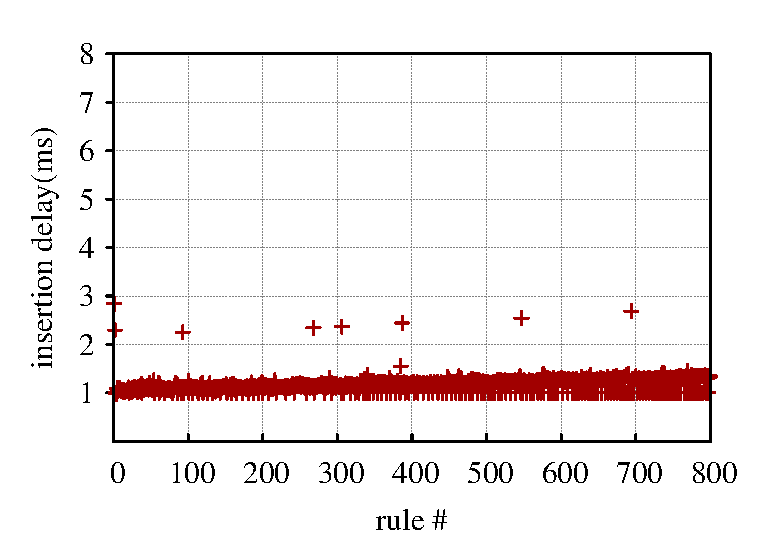
\includegraphics[width=.33\linewidth]{./figs/jan27_intel_same_burst_800.eps}}\hfill
%\subfloat[burst size 200, same priority.\label{fig:intel_burst_200_same_pri}]
%  {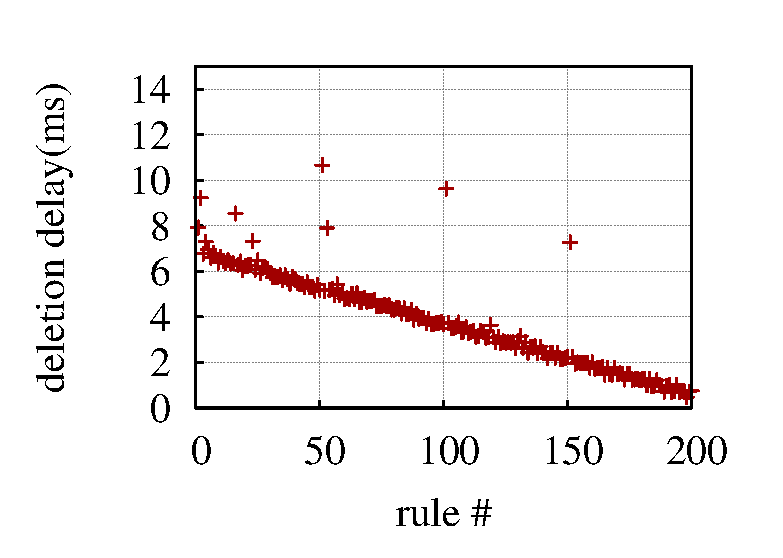
\includegraphics[width=.24\linewidth]{./figs/jan27_intel_same_burst_200.eps}}\hfill
\subfloat[burst size 800, incr. priority\label{fig:intel_burst_800_incr_pri}]
  {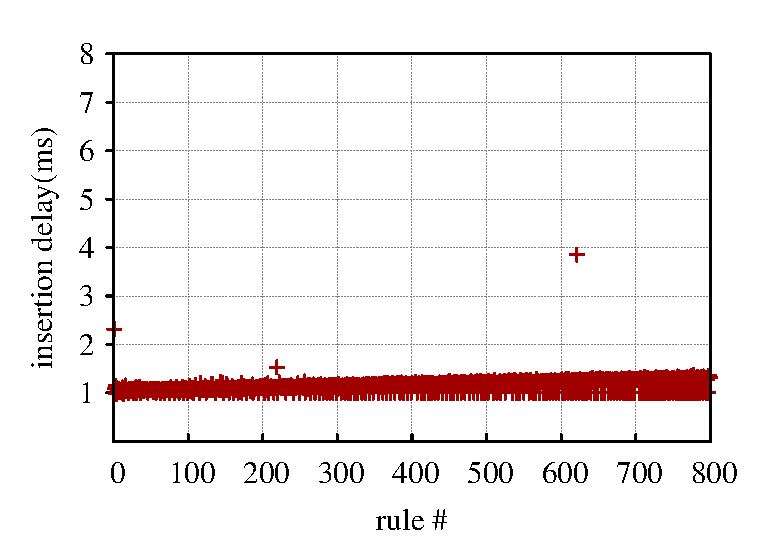
\includegraphics[width=.49\linewidth]{./figs/jan27_intel_incr_burst_800.eps}}\hfill
\subfloat[burst size 800, decr. priority\label{fig:intel_burst_800_decr_pri}]
 {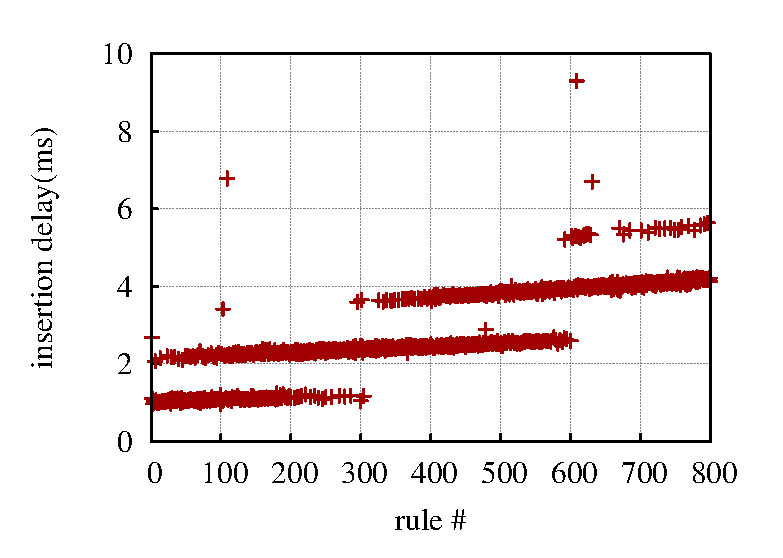
\includegraphics[width=.49\linewidth]{figs/jan27_intel_empty_800L_decr_delta.eps}}
%\subfloat[burst size 200, decreasing priority.\label{fig:intel_burst_200_incr_pri}]
%  {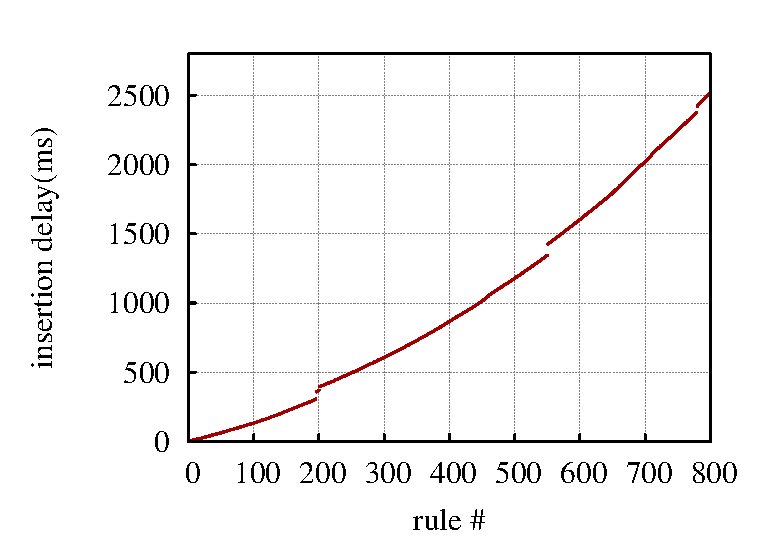
\includegraphics[width=.24\linewidth]{figs/jan27_intel_3200H_800L_decr_real.eps}
\topcompactcaption{{\bf Intel} priority per-rule {\bf insert}
%: (a) burst size
%  100, same priority (b) burst size 200, same priority (c) burst size 100,
%  increasing priority (d) burst size 200, increasing priority {\bf TODO: (e) burst size
%  100, decreasing priority (f) burst size 200, decreasing priority; SHOW the
%  priority effect}
} 
\label{fig:priority-intel-insert}
\end{figure}

\emph{\Intel, same priority.} %Figure~\ref{fig:priority-intel-insert}(a)
For $B=800$ on \Intel\footnote{We present results for a larger value of $B$ 
because the flow table size on \Intel is larger (\tabref{switch_para}).} we see that the per-rule
insertion delay is similar across the 800 rules, with a median of 1.17ms and
standard deviation of 0.16ms (not shown). 
% \aaron{It is odd to show results for B=100 and B=200 for \BroadcomOne, but B=800 for Intel? Do we have higher values of B (e.g., B=600) for \BroadcomOne, so we can use the same B value(e.g., B=600) for both?} 
The results for other values of $B$ are similar. Thus, similar to
\BroadcomOne, \BroadcomThree, and \IBM same priority rule insertion delay does 
not vary with burst size on \Intel. 
%The result for $B=200$ in
%Figure~\ref{fig:priority-intel-insert}(b) shows a similar trend with a
%median delay of xx ms and a standard deviation of
%xx. \aditya{the two sets of lines is interesting and merits
%  discussion!} Thus, similar to Broadcom, same priority rule insertion
%delay does not vary with burst size on Intel.
% we see that the
% same-priority rules isinsertion of a higher priority rule is totally unimpacted by the lower
% priority rules inserted immediately ahead of it. 
% priority rule insertion delay does not vary with burst size on Intel,
% similar to Broadcom.

\emph{\Intel, increasing priority.} %\aditya{graphs for this are missing}
\figref{fig:intel_burst_800_incr_pri} shows per-rule latencies for
$B=800$. \emph{Surprisingly}, in contrast with \BroadcomOne,
\BroadcomThree, and \IBM, the per rule
insertion delay among the rules is more or less the same, with a
median of 1.18ms and a standard deviation of 1.08ms.  We see similar
results for other values of $B$. This shows that the \Intel TCAM architecture 
is fundamentally different from \Broadcom. 
%\aditya{is this a hardware  difference? can it not be SDK?} 
%li: yes, hardware 
Rules are ordered in \Intel's TCAM such that higher priority rule insertion
does not displace existing low priority rules. 
%\aditya{why are we talking about displacement here? we did not mention this for
%broadcom} 

\emph{\Intel, decreasing priority.} %\aditya{graphs for this are missing} 
%The insertion delay increases for decreasing priority insertion.  Rule arrangement in
%  TCAM is such that low priority rule insertion causes displacement of high
%  priority rules. \aditya{this does not appear to be true}
\figref{fig:intel_burst_800_decr_pri} shows per-rule insertion latencies for
$B=800$. We see two effects: (1) the latencies alternate between two modes at any
given time, and (2) a step-function effect after every 300 or so
rules. 


A likely explanation for the former is bus buffering. Since rule insertion is 
part  of the switch's control path, it is not really optimized for latency.
The latter effect can be explained as follows: Examining the \Intel switch architecture, we
find that it has 24 slices, $A_1\ldots A_{24}$, and each slice holds 300
flow entries. There exists a consumption order (low-priority first) across
all slices.  Slice $A_i$ stores the $i^{th}$ lowest priority rule group. If
rules are inserted in decreasing priority, $A_1$ is consumed first until it
becomes full. When the next low priority rule is inserted, this causes one
rule to be displaced from $A_1$ to $A_2$.  This happens for each of the next
300 rules, after which cascaded displacements happen: $A_1 \rightarrow A_2
\rightarrow A_3$, and so on. We confirmed this with \Intel.
%\aditya{we dont have a good explanation for 1}

% ; then $A_2$ starts to be consumed. However, due to the
% decreasing order, 299 existing rules in $A_1$ must be moved into $A_2$, and
% then a new inserted rule will be written into slice $A_1$ until it
% becomes full.
%full, and so on. 


%We suspect some rules trigger
%TCAM reordering and some do not. This results in an ON and OFF process that adds
%delay if the process is on.  
%\aditya{the following is weird} We have been working with Intel closely on our
%measurements. The feedback we got 
%from Intel is that their switch firmware has not been optimized to handle rule
%priorities efficiently in all cases.
%\li{are the two modes strictly alternative? Even rule number mode 1, odd rule
%  number mode 2??}

\minisection{Priority and table occupancy combined effects} 
%Given our understanding of the impact of rule priority and table occupancy on
%per-rule insertion latency, we now study their combined impact. 
We now study the combined impact of rule priority and table occupancy.
We conduct two experiments: For the first experiment, the table starts with
$S$ high priority rules, and we insert $B$ low priority rules.  For the
second experiment, the priorities are inverted.
For both experiments, we measure the total time to install all rules in the
burst, $T(r_B)-T(r_1)$.
%burst rule insertion completion time;
%many applications depend on this the metric (\secref{s:apps}). 

\begin{figure}
\subfloat[insert low priority rules into\newline a table with high priority rules\label{fig:bcm_outbound_two_pri_high_low_burstB}]
  {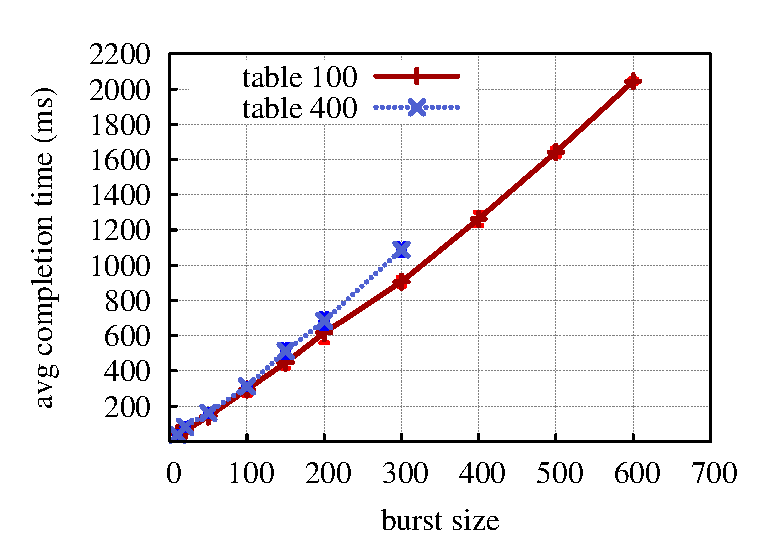
\includegraphics[width=.50\linewidth]{./figs/bcm_two_pri_high_low_burstB.eps}}\hfill
\subfloat[insert high priority rules into a table with low priority rules\label{fig:bcm_outbound_two_pri_low_high_burstB}]
  {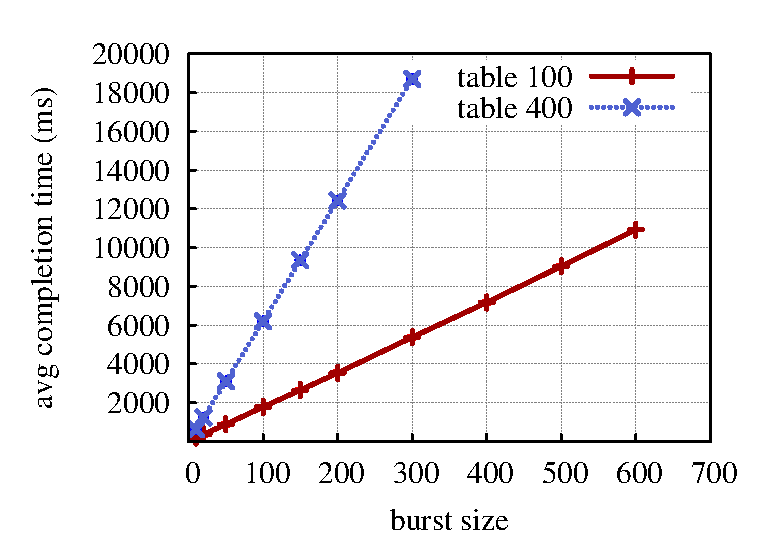
\includegraphics[width=.50\linewidth]{./figs/bcm_two_pri_low_high_burstB.eps}}
\compactcaption{Overall completion time on {\bf \BroadcomOne}.  Initial table occupancy is S high (low) priority rules; insert a burst of low (high) priority rules. Averaged over 5 runs. }
\label{fig:burst-completion-time}
\end{figure}

%We conduct two experiments. With $S$ rules in the table, we insert a burst of $B$ rules. 
%For the first experiment, $S$ has high priority and we insert the burst with low priority. 
%For the second experiment, if it is Broadcom (\BroadcomOne or \BroadcomThree), $S$ has low priority and we insert rules with high priority; if it is Intel, $S$ has high priority and we insert rules in {\em decreasing} priority.

For \BroadcomOne, \BroadcomThree, and \IBM, we expect that as long as the same
number of rules are displaced, the completion time for different values of
$S$ should be the same.
Indeed, from \figref{fig:bcm_outbound_two_pri_high_low_burstB} (for
\BroadcomOne), we see that even with 400 high priority rules in the
table, the insertion delay for the first experiment is no different from the
setting with only 100 high priority rules in the table. In contrast, in
\figref{fig:bcm_outbound_two_pri_low_high_burstB}, newly inserted high
priority rules will displace low priority rules in the table, so when
$S=400$ the completion time is about 3x higher than $S=100$.
%\fixme{added IBM below}
For \IBM (not shown), inserting 300 high priority rules into a table with 400
low priority rules takes more than 20 seconds.  

 
\iffalse
\begin{figure}[!tb]
\centering
\subfloat[decreasing priority\label{fig:intel_burst_100_incr_pri_1}]
  {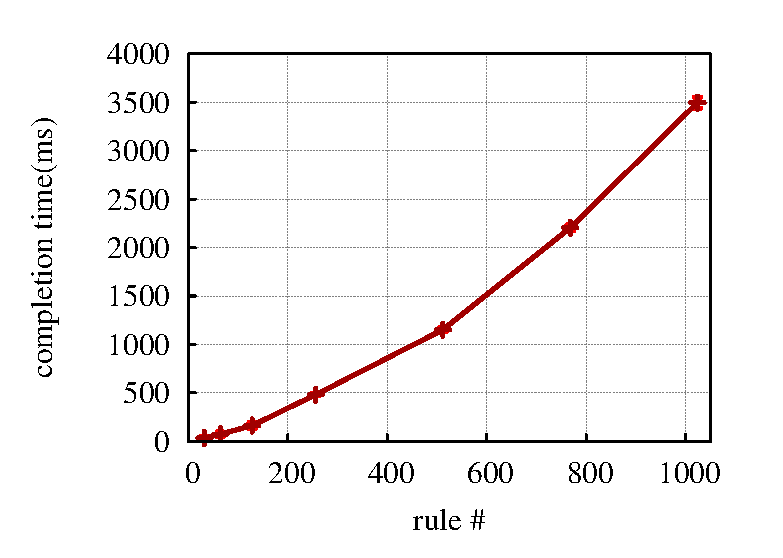
\includegraphics[width=.5\linewidth]{./figs/jan27_intel_decr_burst_size_effect.eps}}\hfill\caption{{\bf Intel} overall completion time} 
\label{fig:priority-intel-insert-more-results}
\end{figure}
\fi

%For \Intel, we also run the same two experiments as for Broadcom. 
For \Intel, the results are similar to same priority rule insertion. This
indicates that \Intel uses different TCAM organization schemes than the
\Broadcom and \IBM switches.  %\fixme{changed}
%optimizes for rule priority better than \BroadcomOne. 
\iffalse
When
we insert in decreasing priority
(\figref{fig:priority-intel-insert-more-results}) the completion time is
about 3.5 seconds, 3x higher than the case of same priority insertion.
\aaron{What is the point of these Intel results?}
\sourav{To show the worst case burst completion time on Intel since it does not have table occupancy effect. But now since the title has been changed from burst completion time to combined effect, I dont think this makes much sense here. }
 \fi
 
\minisection{Summary and root causes}
We observe that: (1) rule complexity does not affect insertion delay; (2)
same priority insertions in \BroadcomOne, \BroadcomThree, \Intel and \IBM are fast
and not affected by flow table occupancy; and (3) priority insertion patterns
can affect insertion delay very differently. For \Intel, increasing priority
insertion is similar to same priority insertion, but decreasing priority 
incurs much higher delay. For \BroadcomThree and \IBM the behavior is inverted:  
decreasing priority insertion is similar to same priority insertion and increasing priority insertion incurs higher delay. For \BroadcomOne, 
insertions with different priority patterns are all much higher than
insertions with same priority. 

Key root causes for observed latencies are: (1) how rules are organized in the TCAM, and (2) the number of slices. {\em Both of these are intrinsically tied to switch hardware.} Even in the best case (\Intel), per-rule insertion latency of 1ms is higher than what native TCAM hardware can support (100M updates/s~\cite{estan:private}). Thus, in addition to the above two causes, there appears to be an {\em intrinsic switch software overhead} contributing to all latencies.

%\aditya{the following is weird} The feedbacks we got from both vendors are that
%their switch firmware has not been 
%optimized for rule priority. 

%\aditya{root causes is incomplete}

\iffalse
Each slice can hold 300 flow entries,
       Also, there exists a consumption order (low-priority first!) across all slices:
       A-slice: the lowest priority rule group, 
       B-slice: the second lowest priority rule group, ….etc  
       In such a case, if the flow rules are inserted in the decreasing priority order,
        A-slice will be first consumed until it becomes full.
        When A-slice is full, B-slice starts to be consumed.
        However, due to the decreasing order, 
       299 existing rules in A-slice must be moved into B-slice
       and then a new inserted rule will be written into A-slice.
       Until B-slice becomes full, and so on.

Based on a phone conversation:
The organization of the TCAM structure is 24 slices x 1024 lines x 36b. There is
also a remap stage between slices 12 and 13. For exact matching 12-tuple
conditions the lookup is split between the 2 halves (pre and post remap stage)
12 slices are used for each of the 12-tuple lookups. Under these conditions then
the OpenFlow table would be limited to 4 groups of 1K entries (4K total). 
If the Key used fewer tuples, or if it could be wild carded the maximum entries
in the TCAM block would be up to 24K. 
There is also an SRAM based Binary Search Tree (longest Prefix match). This is
organized as 4 slices x 16K entries x 32b. If this table is combined with the
TCAM then the maximum flow table size could be as large as 88K entries
(depending on Key size). 
\fi
% LocalWords:  Broadcom TODO Keqiang TCAM feedbacks

\subsubsection{Modification Latency}

We now study  modification operations. As before, we experiment with bursts of rules. Modification latency is defined similar to insertion.

\minisection{\bf Table occupancy} To study the impact of table
occupancy, we pre-insert $S$ rules into a switch,
%(simple rules as before),
all with the same priority. We then modify one rule at a time by changing the
rule's output port, sending modification requests back to back. 

\begin{figure}[!tb]
\centering
\subfloat[100 rules in table \label{fig:bcm_mod_same_burst_100}]
  {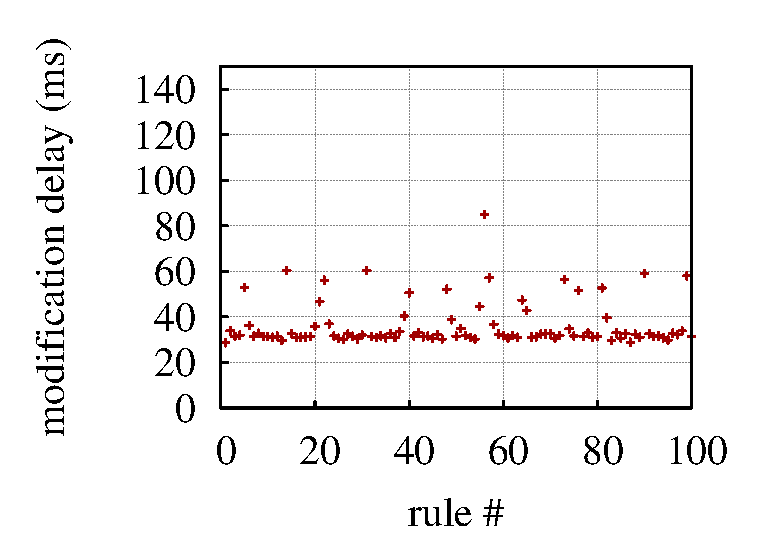
\includegraphics[width=.5\linewidth]{./figs/jan27_bcm_mod_same_burst_100_imc.eps}}\hfill
%\subfloat[burst size 100, increasing priority.\label{fig:bcm_mod_incr_burst_100}]
%  {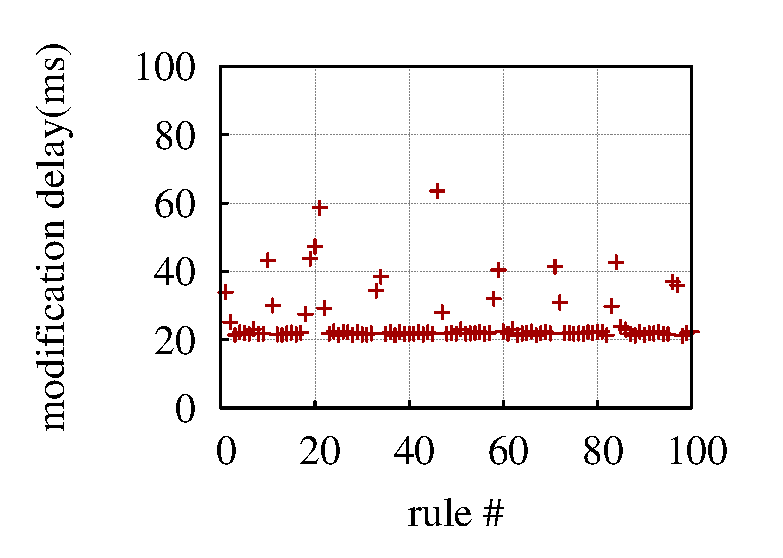
\includegraphics[width=.24\linewidth]{./figs/jan27_bcm_mod_incr_burst_100.eps}}\hfill
%\subfloat[burst size 100, decreasing priority.\label{fig:bcm_mod_decr_burst_100}]
%  {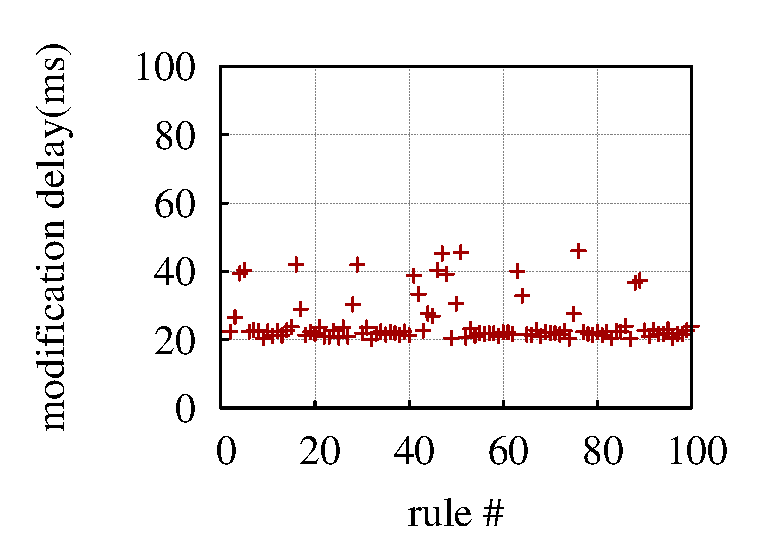
\includegraphics[width=.24\linewidth]{./figs/jan27_bcm_mod_decr_burst_100.eps}}\hfill
\subfloat[200 rules in table \label{fig:bcm_mod_same_burst_200}]
  {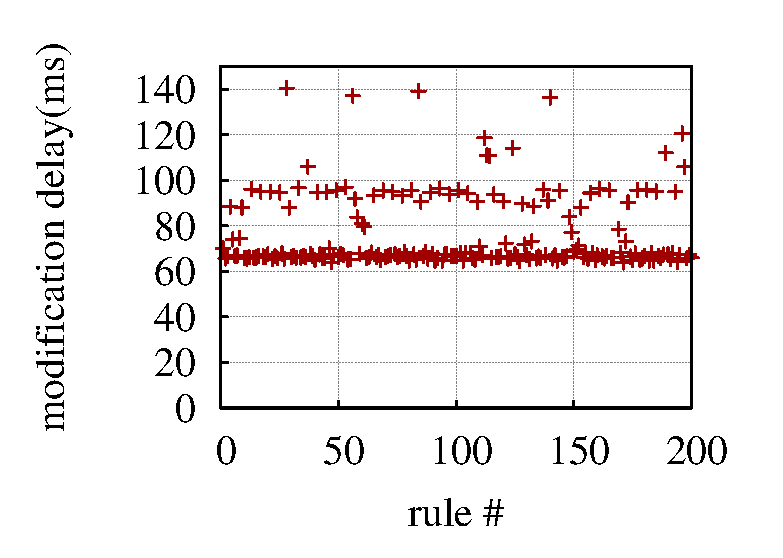
\includegraphics[width=.5\linewidth]{./figs/jan27_bcm_mod_same_burst_200.eps}}
\compactcaption{{\bf \BroadcomOne} per-rule {\bf mod.} latency, same priority}
\label{fig:occupancy-broadcom-modify}
\end{figure}
 
Per-rule modification delay for \BroadcomOne when $S=100$ and $S=200$ are shown in
\figsref{fig:bcm_mod_same_burst_100}{fig:bcm_mod_same_burst_200}, respectively. We
see that the per-rule delay
is more than 30 ms for $S=100$. When we double the number of rules,
$S=200$, latency doubles as well. It grows
linearly with $S$ (not shown). Note that
this latency is much higher than the corresponding
insertion latency (3.12ms per rule) (\S\ref{s:meas_insert}).
%\fixme{IBM added}
\IBM's per-rule modification latency is also affected significantly by the table occupancy---
the per-rule modification latencies for $S=100$ and $S=200$ are 18.77ms and 37.13ms, respectively.
 
\iffalse
\begin{figure}[!tb]
  \centering \subfloat[100 rules in table \label{fig:intel_mod_same_burst_100}]
  {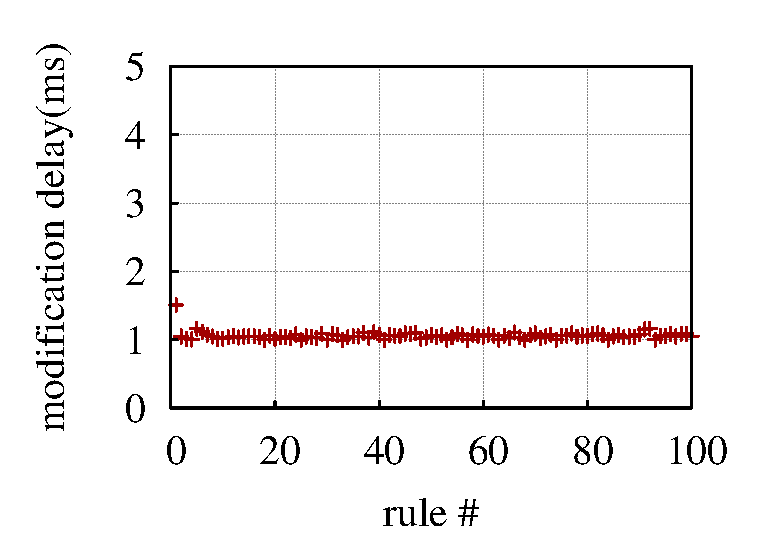
\includegraphics[width=.5\linewidth]{./figs/jan27_intel_mod_same_burst_100.eps}}\hfill
%\subfloat[burst size 100, increasing priority.\label{fig:intel_mod_incr_burst_100}]
%  {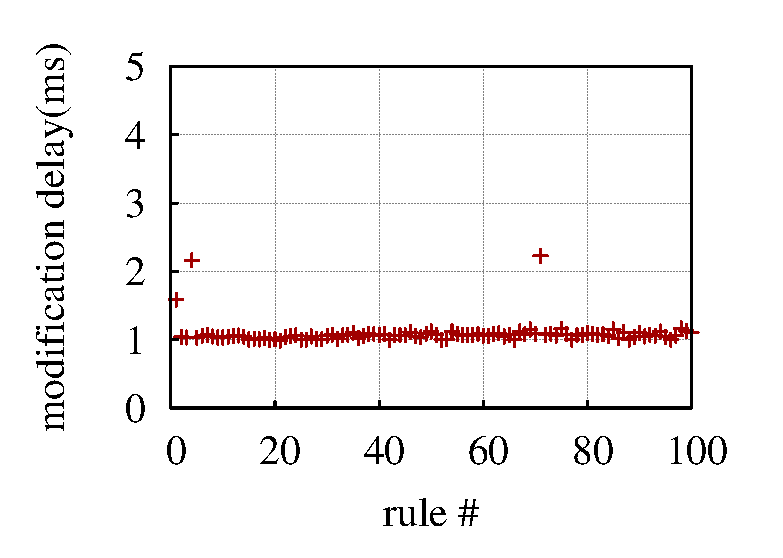
\includegraphics[width=.24\linewidth]{./figs/jan27_intel_mod_incr_burst_100.eps}}\hfill
%\subfloat[burst size 100, decreasing priority.\label{fig:intel_mod_decr_burst_100}]
%  {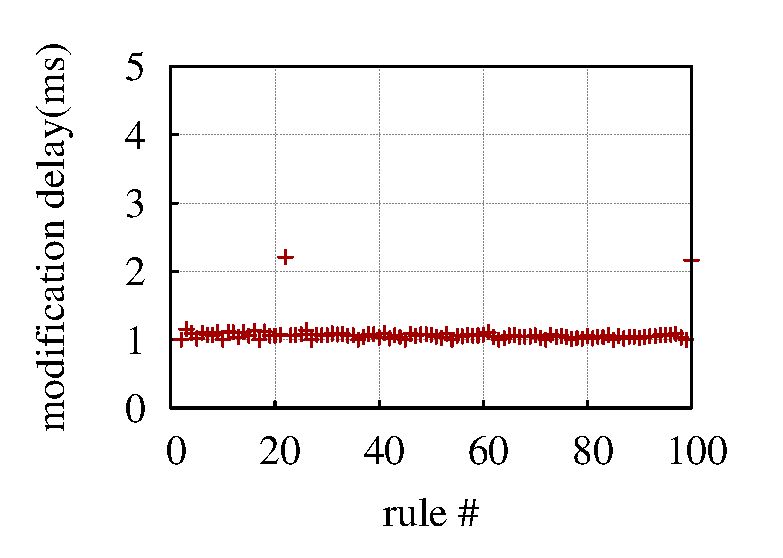
\includegraphics[width=.24\linewidth]{./figs/jan27_intel_mod_decr_burst_100.eps}}\hfill
\subfloat[200 rules in table \label{fig:intel_mod_same_burst_200}]
  {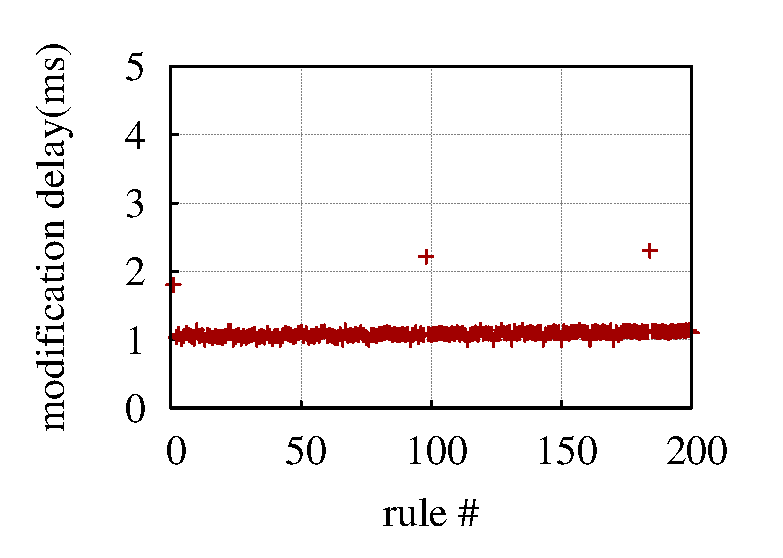
\includegraphics[width=.5\linewidth]{./figs/jan27_intel_mod_same_burst_200.eps}}
\compactcaption{{\bf \Intel} per-rule {\bf mod.} latency, same priority}
\label{fig:occupancy-intel-modify}
\end{figure}
\fi
%The results for $S=100,200$ for Intel are shown in
%Figure~\ref{fig:occupancy-intel-modify}. 
%Sourav commented
%For Intel, the modification delay for $S=100,200$ is around 1 ms
%(standard deviation 0.06) for all modified rules, similar to insertion
%in Figure~\ref{fig:priority-intel-insert}.
%delay with same priority,  in contrast with
%\BroadcomOne. 
% the modification delay is around 1 ms, which is the same as
% the insertion delay when all rules have same priority
% (\S\ref{s:meas_insert}).
% The results are the same for higher values of
% $S$.

In contrast, \Intel and \BroadcomThree  have lower modification delay,
and it does not vary with table occupancy. For \Intel (\BroadcomThree) the
per-rule modification delay for both $S=100$ and $S=200$ is around 1 ms (2ms)
for all modified rules, similar to (2X more than) same priority insertion delay. 

%\aditya{I changed the previous sentences. Check!!}
%%  For \BroadcomThree the average modification delay (standard deviation) for $S=100$ and $S=200$ is 2.19 (1.82) and 2.95 (2.29) respectively.
%For \BroadcomThree the modification delay is highly variable and is 
%related with table occupancy. For example, modifying 200 %rules in a table with 200 and 500 rules takes 449 and %4984 msec respectively. 

\minisection{Rule Priority} We conduct two experiments on each switch to
study the impact of rule priority. In
each experiment, we insert $B$ rules into an empty table ($S = 0$). In the 
{\em increasing} priority experiments, the rules in the table each have a
unique priority, and we send back-to-back modification requests for
rules in increasing priority order. We do the opposite in the {\em
decreasing priority} experiment. We vary $B$.%  across
% experiments. Note that the {\em same priority} experiment here is
% exactly the same as the table occupancy experiment above; hence we
% omit it.

\begin{figure}[!tb]
\centering
%\subfloat[burst size 100, same priority.\label{fig:bcm_mod_same_burst_100}]
%  {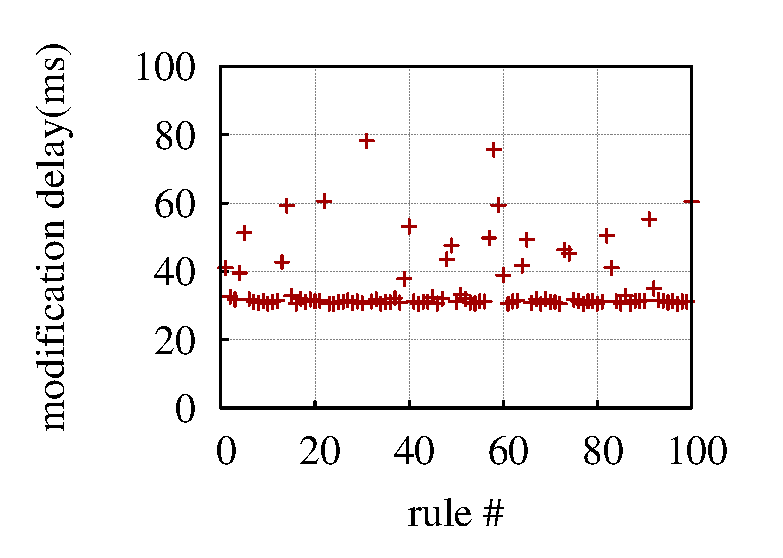
\includegraphics[width=.5\linewidth]{./figs/jan27_bcm_mod_same_burst_100.eps}}\hfill
\subfloat[burst size 100, incr. priority\label{fig:bcm_mod_incr_burst_100}]
  {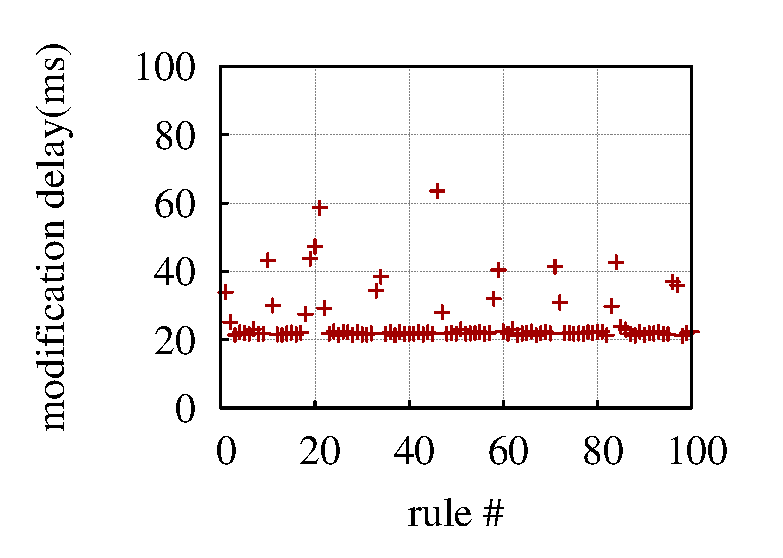
\includegraphics[width=.5\linewidth]{./figs/jan27_bcm_mod_incr_burst_100.eps}}\hfill
\subfloat[burst size 100, decr. priority\label{fig:bcm_mod_decr_burst_100}]
  {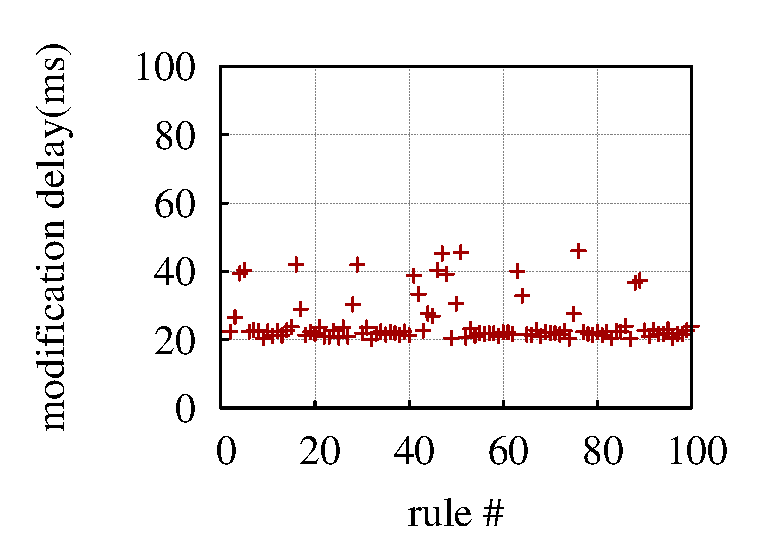
\includegraphics[width=.5\linewidth]{./figs/jan27_bcm_mod_decr_burst_100.eps}}\hfill
%\subfloat[burst size 200, same priority.\label{fig:bcm_mod_same_burst_200}]
%  {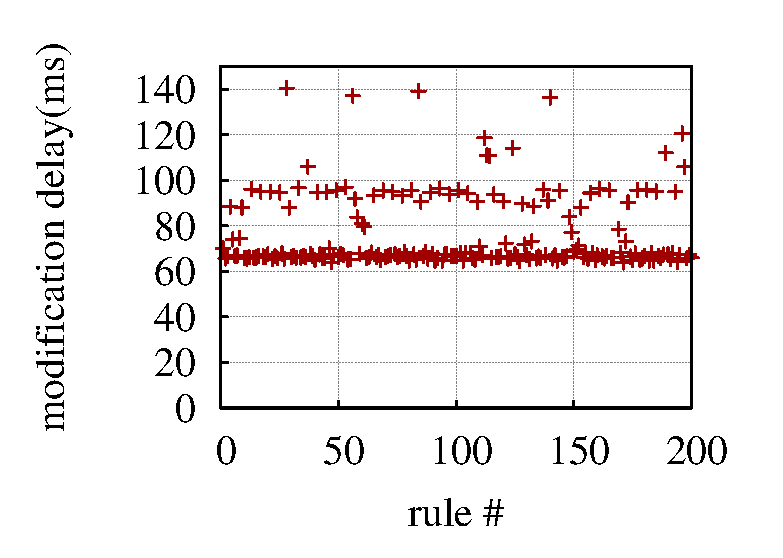
\includegraphics[width=.5\linewidth]{./figs/jan27_bcm_mod_same_burst_200.eps}}
\compactcaption{{\bf \BroadcomOne} priority per-rule {\bf modification} latency}
\label{fig:priority-broadcom-modify}
\end{figure}

%\emph{\BroadcomOne: increasing/decreasing priority.}
\figsref{fig:bcm_mod_incr_burst_100}{fig:bcm_mod_decr_burst_100} show the results for the increasing and decreasing priority experiments, respectively, for
$B=100$ on \BroadcomOne. In both cases, we see: (1) the per-rule modification delay is similar
across the rules, with a median of 25.10ms and a standard deviation of
6.74ms, and (2) the latencies are identical across the experiments. 
We similarly observe that priority does not affect modification delay in
\BroadcomThree, \Intel and \IBM (not shown).
% Again, the
% latencies are  much larger than insertion with same priority, 25 ms vs 3 ms.
%\aditya{this is not true! bcm insertion latencies are also high!} 
%li: add same priority, fixed, right?
%We observed that the latencies grew with $B$ for both experiments.
% increasing and decreasing
% priority experiments.

% Figure~\ref{fig:priority-broadcom-modify}-d shows the results for
% $B=200$, and again the per rule latency is about twice as high as that
% for $B=100$. 
% % per-rule modification delay for 200 rules has a median 60 (xx) ms and
% % standard deviation xx. The modification time is significant impacted
% % by the number of rules in the table.

% \emph{Broadcom: decreasing priority.}  We modify in both increasing rule
%   priority and decreasing rule priority. As shown in
%   Figure~\ref{fig:priority-broadcom-insert}-b,c, the per rule modification delay
%   is not affected by rule priority. Their median delay is xx and xx respectively
%   with standard deviation xx and xx.

%We next describe our measurement results on Intel. 
\iffalse
\begin{figure}[!tb]
\centering
%\subfloat[burst size 100, same priority.\label{fig:intel_mod_same_burst_100}]
%  {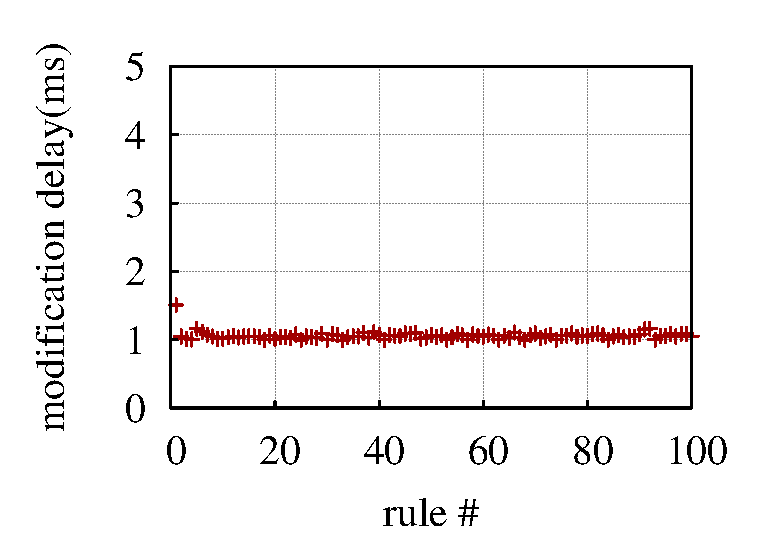
\includegraphics[width=.5\linewidth]{./figs/jan27_intel_mod_same_burst_100.eps}}\hfill
\subfloat[burst size 100, increasing priority.\label{fig:intel_mod_incr_burst_100}]
  {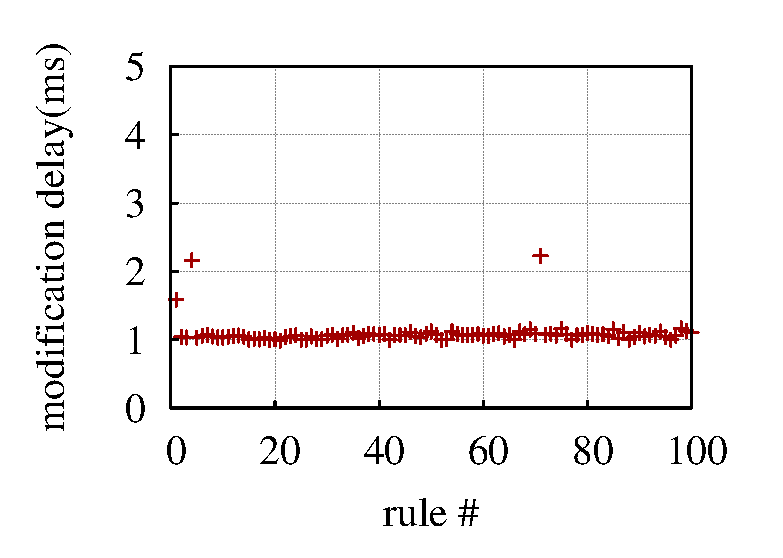
\includegraphics[width=.5\linewidth]{./figs/jan27_intel_mod_incr_burst_100.eps}}\hfill
 \subfloat[burst size 100, decreasing priority.\label{fig:intel_mod_decr_burst_100}]
  {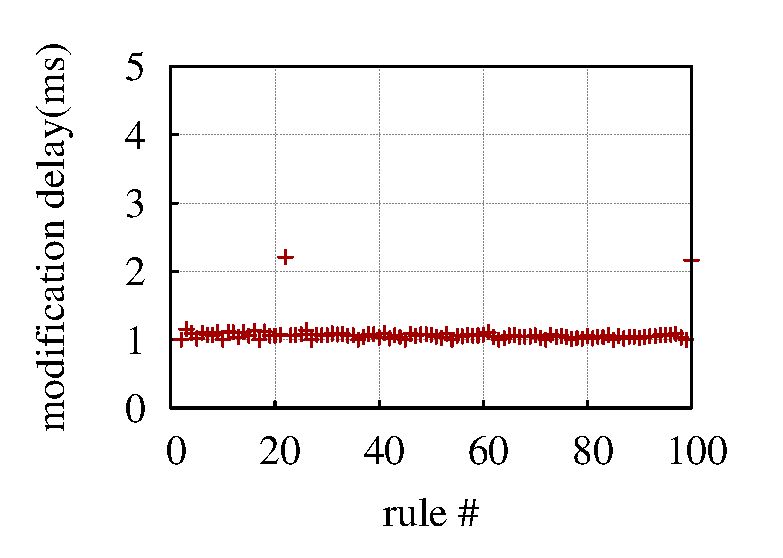
\includegraphics[width=.5\linewidth]{./figs/jan27_intel_mod_decr_burst_100.eps}}\hfill
%\subfloat[burst size 200, same priority.\label{fig:intel_mod_same_burst_200}]
%  {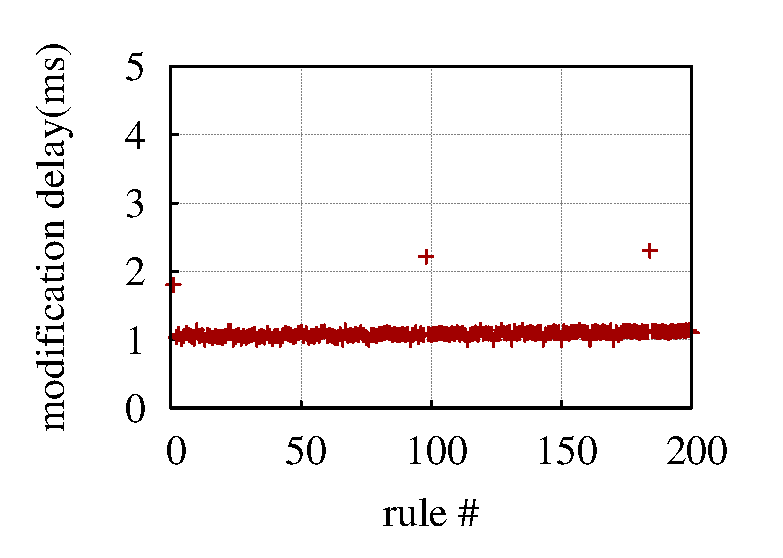
\includegraphics[width=.5\linewidth]{./figs/jan27_intel_mod_same_burst_200.eps}}
\caption{{\bf Intel} priority per-rule {\bf modification} latency results}
\label{fig:priority-intel-modify}
\end{figure}
\fi

%{\em Intel increasing/decreasing priority.} 
%Figure~\ref{fig:priority-intel-modify} shows the result for $B=100$ on
%Intel.
% , similar to insertion delay without
% priority.  We also tried other B values and the results are similar (omitted for brevity).


\minisection{Summary and root causes}
%Given our table occupancy and rule priority results, 
We conclude that the per-rule modification latency on \BroadcomOne and \IBM is 
impacted purely by table occupancy, not by rule priority structure.
For \BroadcomThree and \Intel, the per-rule modification delay 
%is 1 ms respectively 
is independent of rule priority, table occupancy, and burst size;
\BroadcomThree's per-rule modification delay is 2X higher than insertion.
%For \BroadcomThree, the modification delay is independent of rule priority but 
%is highly variable and is          
%related with table occupancy. The root cause of the variable and larger modification delay on 
%\BroadcomOne and \BroadcomThree is that modification involves insertion and deletion operation and it causes
%TCAM reorganization.

%We observe that flow rule priority do
%not impact modification delay. Modification delay in \BroadcomOne and \BroadcomThree is a
%function of table occupancy, whereas this is not the case for Intel where modification is as fast as insertion. 
Conversations with Broadcom indicated that TCAM modification should ideally be fast and independent of table size, 
so the underlying cause appears to be less optimized switch software in \BroadcomOne. Indeed, our measurements with \BroadcomThree show that this issue has (at least partly) been fixed.

% However, for Broadcom, the modification delay is much higher
% than rule insertion delay with same priority. For Intel, the modification delay
% is similar to rule insertion delay with same priority. 

% \aditya{missing causes!}


% LocalWords:  pre Broadcom

\subsubsection{Deletion Latency}
We now estimate the impact of rule deletions.
We use bursts of operations as before.
Denote
$T(r_i)$ as the first time we stopped observing packets matching rule $r_i$
from the intended port of the rule action. We define deletion latency
as $T(r_i)-T(r_{i-1})$.

\begin{figure}[!tb]
\centering
\subfloat[100 rules in table \label{fig:bcm_del_same_burst_100}]
  {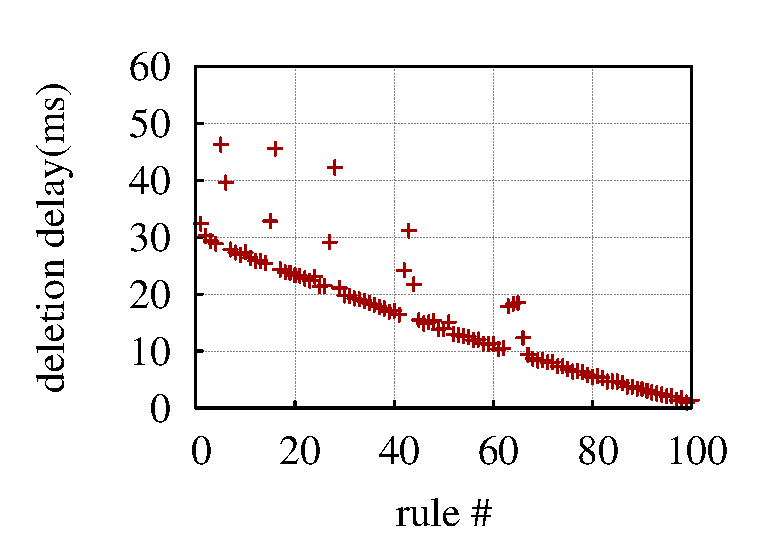
\includegraphics[width=.50\linewidth]{./figs/jan27_bcm_del_same_burst_100.eps}}\hfill
%\subfloat[burst size 100, increasing priority.\label{fig:bcm_del_incr_burst_100}]
%  {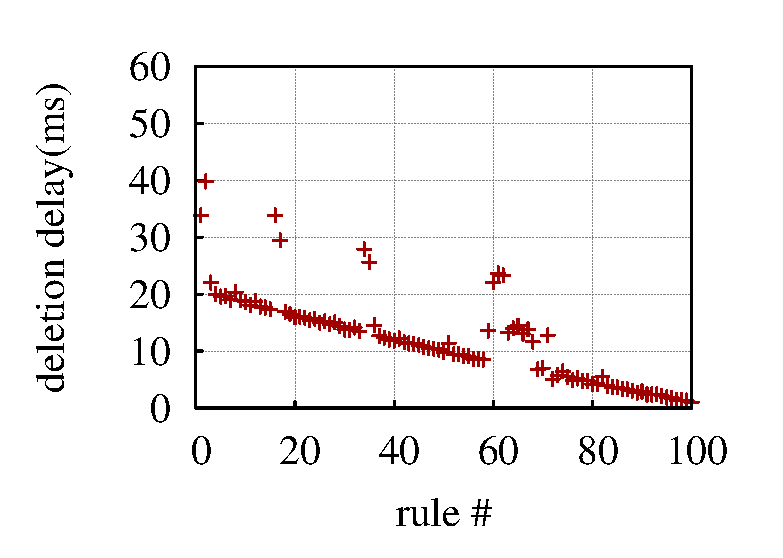
\includegraphics[width=.30\linewidth]{./figs/jan27_bcm_del_incr_burst_100.eps}}\hfill
\subfloat[200 rules in table \label{fig:bcm_del_same_burst_200}]
  {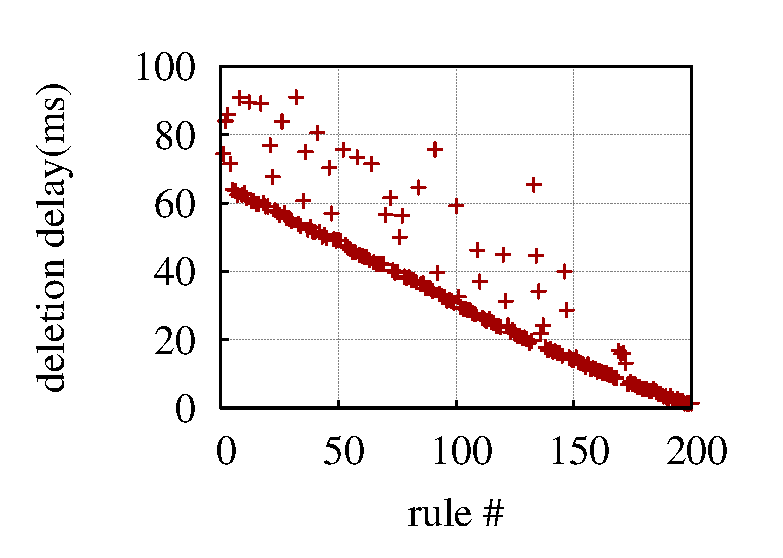
\includegraphics[width=.50\linewidth] {./figs/jan27_bcm_del_same_burst_200.eps}}
\compactcaption{ {\bf \BroadcomOne} per-rule {\bf del.} latency, same priority}
\label{fig:occupancy-broadcom-deletion}
\end{figure}

\begin{figure}[!tb]
\centering
\subfloat[100 rules in table\label{fig:intel_del_same_burst_100}]
  {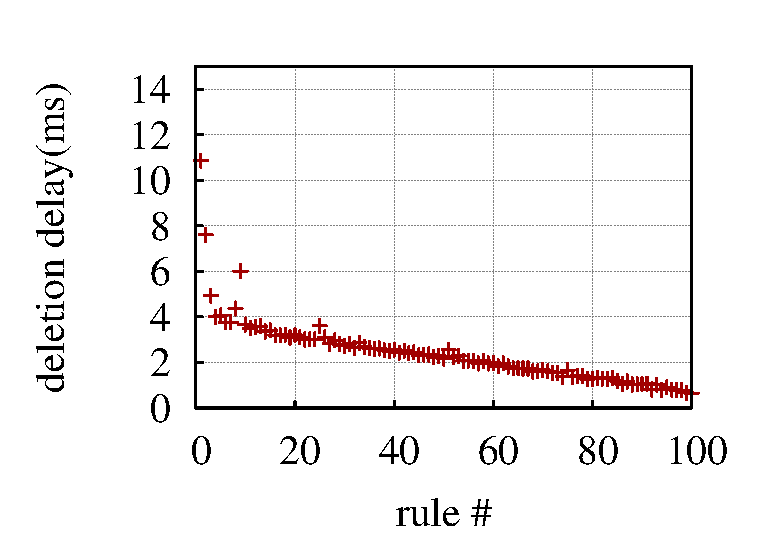
\includegraphics[width=.50\linewidth]{./figs/jan27_intel_del_same_burst_100.eps}}\hfill
%\subfloat[burst size 100, increasing priority.\label{fig:intel_del_incr_burst_100}]
%  {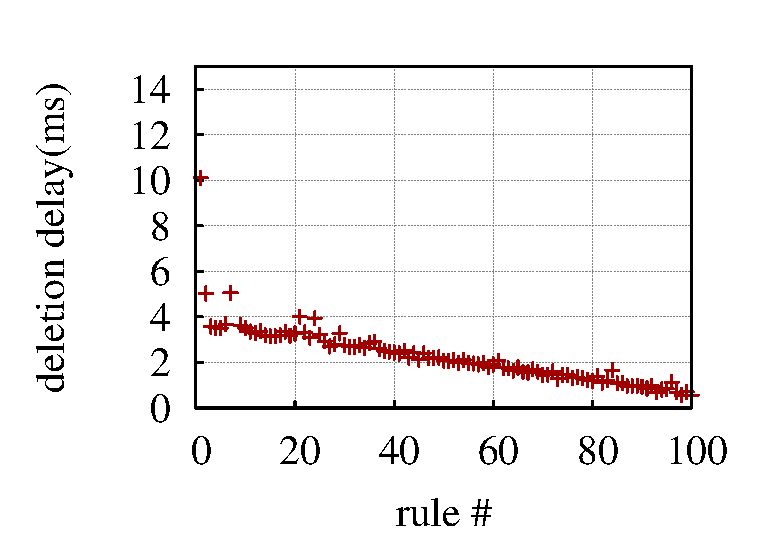
\includegraphics[width=.30\linewidth]{./figs/jan27_intel_del_incr_burst_100.eps}}\hfill
\subfloat[200 rules in table \label{fig:intel_del_same_burst_200}]
  {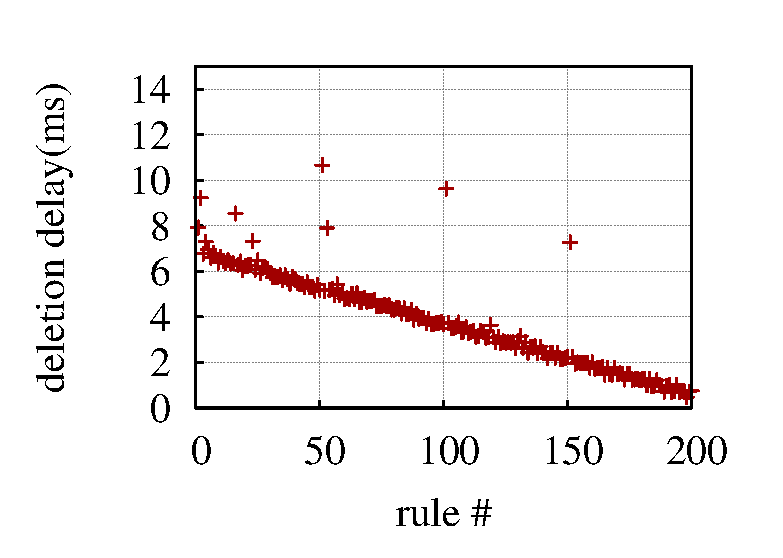
\includegraphics[width=.50\linewidth]{./figs/jan27_intel_same_burst_200.eps}}
\compactcaption{{\bf \Intel} per-rule {\bf del.} latency, same priority}
\label{fig:occupancy-intel-deletion}
\end{figure}

\minisection{Table Occupancy} We pre-insert $S$ rules into a switch, all with
the same priority. We then delete one rule at a time, sending deletion
requests back-to-back. The results for \BroadcomOne at $S=100$ and $S=200$
are shown in \figsref{fig:bcm_del_same_burst_100}{fig:bcm_del_same_burst_200},
respectively. We see that per rule deletion delay decreases as the table occupancy drops. We see a similar trend for Intel (\figsref{fig:intel_del_same_burst_100}{fig:intel_del_same_burst_200}) and \BroadcomThree (figure not shown).

%  and
% ~\ref{fig:occupancy-intel-deletion}, the per rule deletion delay
% decreases as the table occupancy drops.


\begin{figure}[!tb]
\centering
% \subfloat[burst size 100, same priority.\label{fig:bcm_del_same_burst_100}]
%   {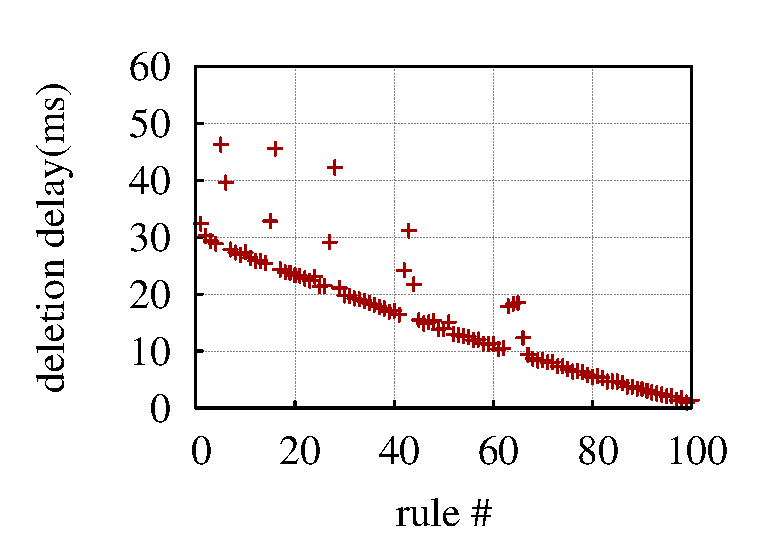
\includegraphics[width=.30\linewidth]{./figs/jan27_bcm_del_same_burst_100.eps}}\hfill
\subfloat[increasing priority\label{fig:bcm_del_incr_burst_100}]
  {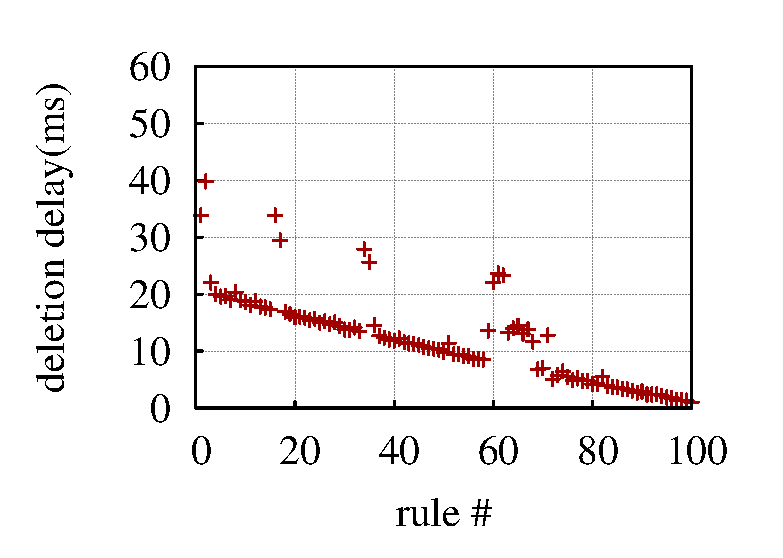
\includegraphics[width=.50\linewidth]{./figs/jan27_bcm_del_incr_burst_100.eps}}\hfill
\subfloat[decreasing priority\label{fig:bcm_del_decr_burst_100}]
  {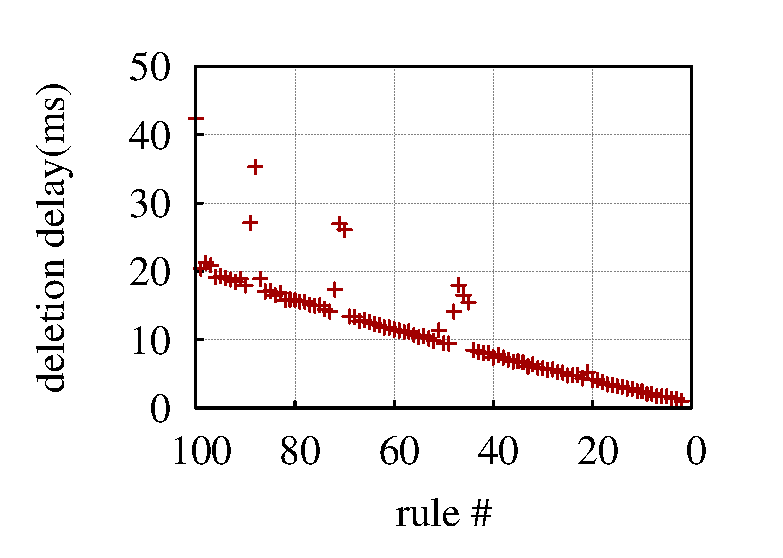
\includegraphics[width=.50\linewidth]{./figs/jan27_bcm_del_decr_burst_100.eps}}
\compactcaption{{\bf \BroadcomOne} priority per-rule {\bf del.} latency, 
    B=100}
\label{fig:priority-broadcom-deletion}
\end{figure}

\begin{figure}[!tb]
\centering
%\subfloat[burst size 100, same priority.\label{fig:jan27_intel_del_same_burst_100}]
%  {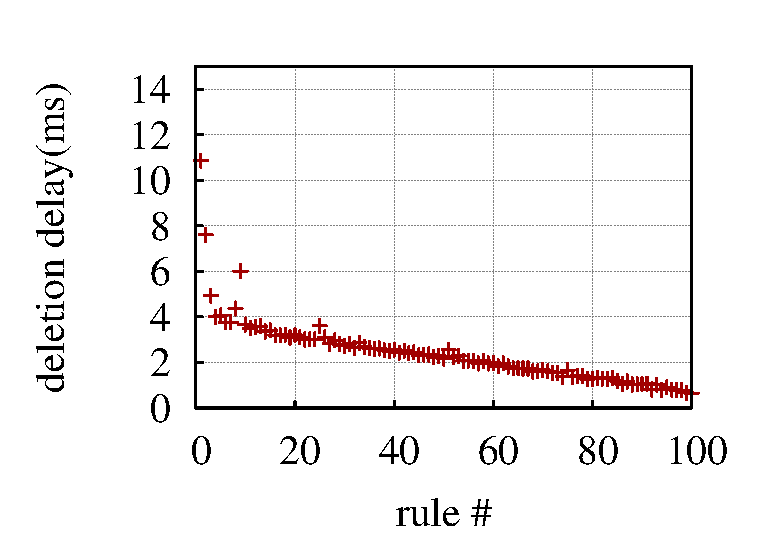
\includegraphics[width=.24\linewidth]{./figs/jan27_intel_del_same_burst_100.eps}}\hfill
%\subfloat[burst size 100, increasing priority.\label{fig:jan27_intel_del_incr_burst_100}]
%  {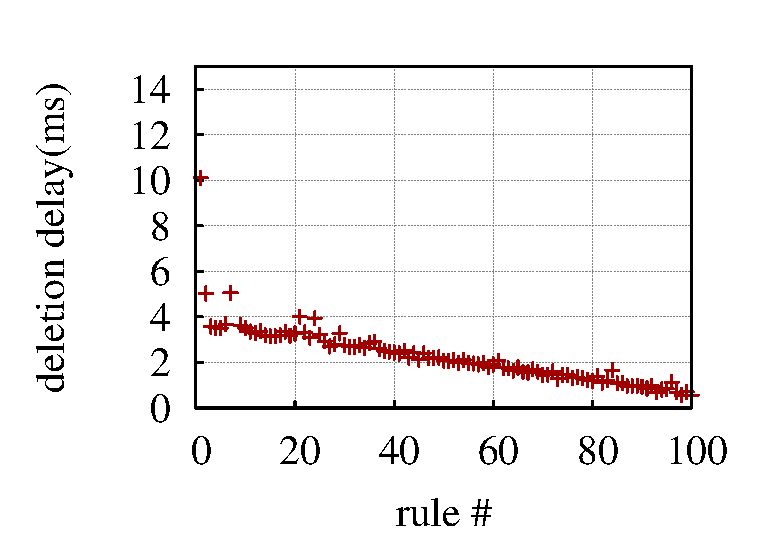
\includegraphics[width=.24\linewidth]{./figs/jan27_intel_del_incr_burst_100.eps}}\hfill
%\subfloat[burst size 100, decreasing priority.\label{fig:jan27_intel_del_decr_burst_100}]
%  {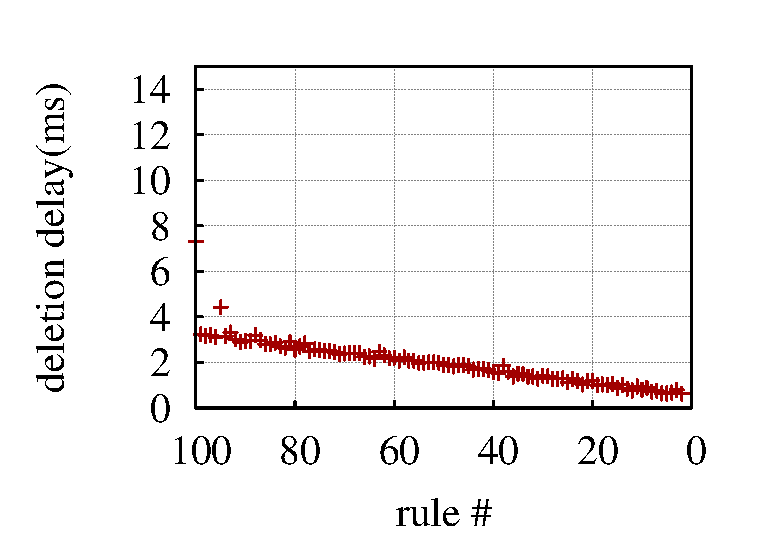
\includegraphics[width=.24\linewidth]{./figs/jan27_intel_del_decr_burst_100.eps}

% \subfloat[burst size 100, same priority.\label{fig:intel_intel_del_same_burst_100}]
%   {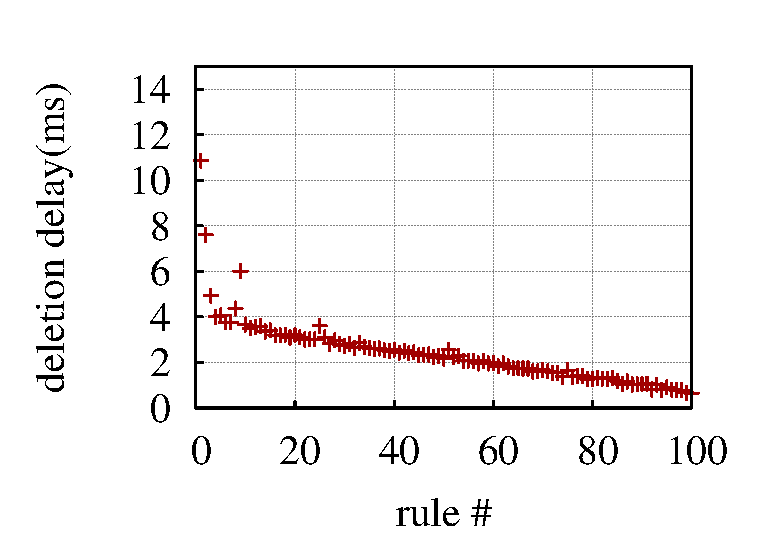
\includegraphics[width=.30\linewidth]{./figs/jan27_intel_del_same_burst_100.eps}}\hfill
\subfloat[increasing priority\label{fig:intel_del_incr_burst_100}]
  {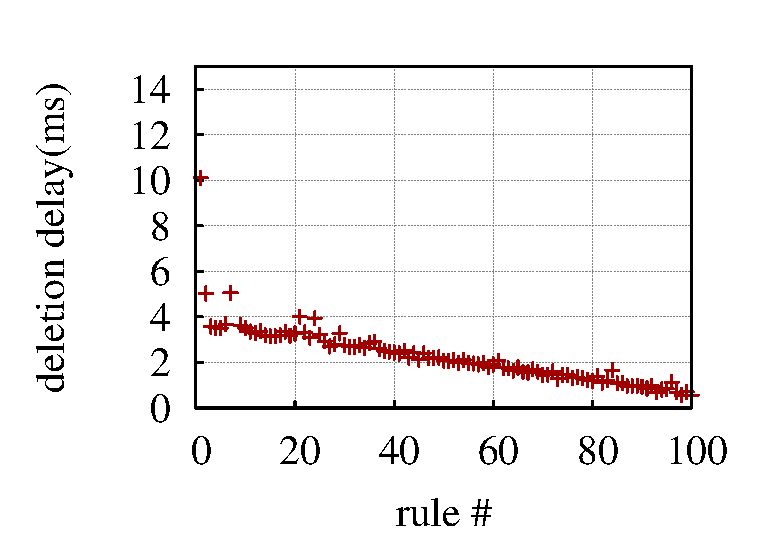
\includegraphics[width=.50\linewidth]{./figs/jan27_intel_del_incr_burst_100.eps}}\hfill
\subfloat[decreasing priority\label{fig:intel_del_decr_burst_100}]
  {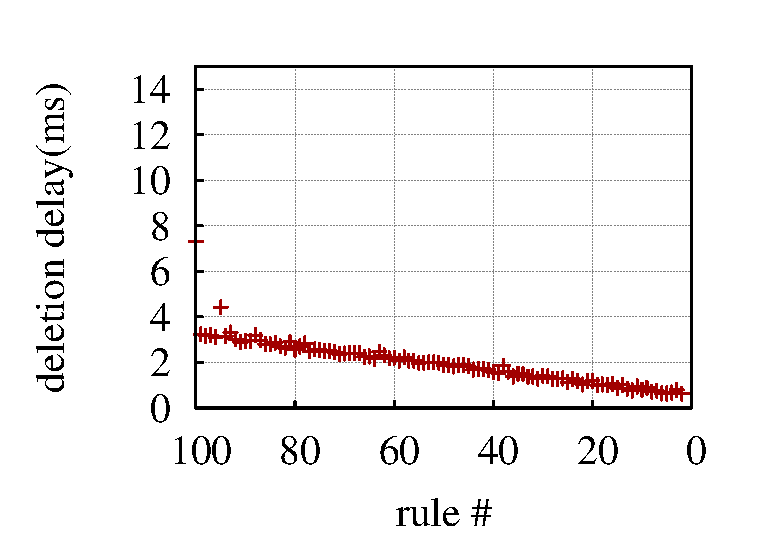
\includegraphics[width=.50\linewidth]{./figs/jan27_intel_del_decr_burst_100.eps}}

\compactcaption{{\bf Intel} priority per-rule {\bf del.} latency, B=100}
\label{fig:priority-intel-deletion}
\end{figure}


\minisection{Rule Priorities} We start with $B$ existing rules in the switch, 
and delete one rule at a time
%,``with'' and ``without priority''. In the former case, 
%we delete rules 
in increasing and decreasing priority order. 
For \BroadcomOne (\figref{fig:priority-broadcom-deletion}), \BroadcomThree
(figure not shown) and Intel (\figref{fig:priority-intel-deletion}), deletion 
is not affected by the priorities of rules in the table or the order of
deletion. %\aaron{Where are the without priority results?}


\minisection{\bf Root cause} Since deletion delay decreases with rule number 
in all cases, we conclude that deletion is incurring TCAM reordering.
% We observe that rule priority pattern does not affect deletion delay for both
% Broadcom and Intel. However, flow table occupancy affects deletion delay
% significant. Deletion delay can be much higher than insertion delay with same
% priority. 
% This seems to indicate that deletion incurs TCAM reordering in all
% cases in both switch architectures.
We also observe that processing rule timeouts at the switch does not
noticeably impact \flowmod operations. Given these two observations, we
recommend allowing rules to time out rather than explicitly deleting them, if
possible.

% LocalWords:  pre Broadcom TODO butbound TCAM

\subsubsection{Impact of concurrent switch CPU jobs} 
\begin{figure}
\subfloat[init. table occupancy 0\label{fig:bcm_polling_table0_burst100}]
  {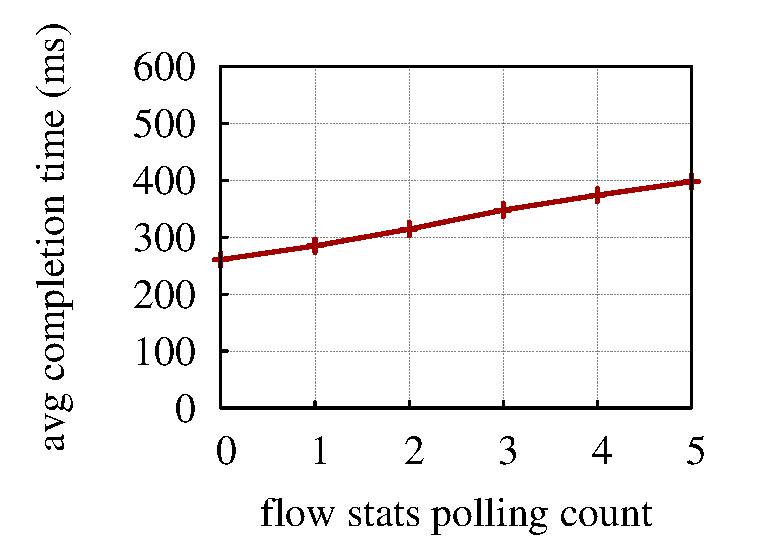
\includegraphics[width=0.25\textwidth]{./figs/bcm_polling_table0_burst100.eps}}
\subfloat[init. table occupancy 500\label{fig:bcm_polling_table500_burst100}]
  {\includegraphics[width=0.25\textwidth]{./figs/bcm_polling_table500_burst100.eps}}\hfill
%\subfloat[controlled-rate mode, rate 50, polling frequency = 1/s\label{fig:bcm_polling_control_50_50_per_polling}]
%  {\includegraphics[width=0.3\textwidth]{./figs/bcm_polling_control_50_50_per_polling.eps}}
\topcompactcaption{Impact of polling on {\bf \BroadcomOne}, B=100}
%    ., simple rules (i.e., only specify destination IP)}
%\caption{{\bf Broadcom} per-rule {\bf insert} latency: impact of polling}
\label{fig:polling}
\end{figure}

We previously showed the impact of \flowmod processing on inbound latency
(\secref{s:measure_inbound}). We now study the impact of statistics
polling on outbound latency. 
%In particular,
%To investigate the impact of concurrent switch CPU activities, 
%we instruct the switch to report flow statistics.
%perform flow statistics queries. 
Figure~\ref{fig:polling} shows that concurrent activities, such as polling
statistics, can have a big impact on insertion delay, especially when table
occupancy is high: e.g., with \BroadcomOne, the total time to insert a 
burst of 100 same priority rules into a table with 500 rules is 853ms when 
two polling events occur during the insertion process, compared to
356ms without polling events.
%If we do not poll, the completion
%time of a burst insertion of 100 rules is 280 (xx) ms. If we poll all rules including
%recently installed 10 times during the burst insertion, the
%completion time becomes 490 (xx) ms. 
%\aditya{isn't this polling rate too high?} \aditya{what is the xx supposed to be?}
%$\li{Are we polling existing rule stats? It seems we also poll newly inserted
%  rule stats. What is polling count? }.
\iffalse
\subsection{Overall burst insertion completion time}
With the understanding of per-rule insertion latency, we present burst rule insertion
completion time as this is the metric many applications such as failover depend
on. 

\begin{figure}
\subfloat[insert low priority rules into\newline a table with high priority rules\label{fig:bcm_outbound_two_pri_high_low_burstB}]
  {\includegraphics[width=.50\linewidth]{./figs/bcm_two_pri_high_low_burstB.eps}}\hfill
\subfloat[insert high priority rules into a table with low priority rules\label{fig:bcm_outbound_two_pri_low_high_burstB}]
  {\includegraphics[width=.50\linewidth]{./figs/bcm_two_pri_low_high_burstB.eps}}
\compactcaption{Overall completion time on {\bf \BroadcomOne}.  Initial table
occupancy is S high (low) priority rules; insert a burst of low (high)
priority rules. Averaged over 5 runs. }
\label{fig:burst-completion-time}
\end{figure}
\fi




\iffalse
\begin{figure}[!tb]
\centering
%\subfloat[burst size 100, same priority.\label{fig:intel_burst_100_same_pri}]
%  {\includegraphics[width=.24\linewidth]{./figs/jan27_intel_same_burst_100.eps}}\hfill
%\subfloat[burst size 200, same priority.\label{fig:intel_burst_200_same_pri}]
%  {\includegraphics[width=.24\linewidth]{./figs/jan27_intel_same_burst_200.eps}}\hfill
%\subfloat[burst size 800 of low priority, table has 3200 high priority rules\label{fig:intel_burst_200_same_pri}]
%\epsfig{file=./figs/Intel_burst_effect_same.eps,width=0.5\textwidth}
%  {\includegraphics[width=.5\linewidth]{./figs/jan27_intel_burst_effect_same.eps}}\hfill %jan27_intel_decr_burst_100.eps
%   {\includegraphics[width=.5\linewidth]{./figs/jan27_intel_3200H_800L_L_to_H_delta.eps}} \hfill
\subfloat[decreasing priority\label{fig:intel_burst_100_incr_pri_1}]
  {\includegraphics[width=.7\linewidth]{./figs/jan27_intel_decr_burst_size_effect.eps}}\hfill %jan27_intel_decr_burst_100.eps
%\subfloat[burst size 200, decreasing priority.\label{fig:intel_burst_200_incr_pri}]
%  {\includegraphics[width=.5\linewidth]{figs/jan27_intel_3200H_800L_decr.eps}}
%\subfloat[burst size 200, decreasing priority.\label{fig:intel_burst_200_decr_pri}]
%  {\includegraphics[width=.24\linewidth]{figs/jan27_intel_decr_burst_size_effect.eps}
\caption{{\bf Intel} overall completion time} 
\label{fig:priority-intel-insert-more-results}
\end{figure}
\fi
%\aditya{Is figure 14a correct? It says same priority}
\iffalse
We conduct two experiments. With $S$ rules in the table, we insert a burst of $B$ rules. 
For the first experiment, $S$ has high priority and we insert the burst with low priority. 
For the second experiment, if it is Broadcom (\BroadcomOne or \BroadcomThree), $S$ has low priority and we insert rules with high priority; 
if it is Intel, $S$ has high priority and we insert rules in {\em decreasing} priority.

For Broadcom, based on our hypothesis, as long as the same number of
rules get displaced, the completion time should be the same. Indeed,
 from \figref{fig:bcm_outbound_two_pri_high_low_burstB} (for \BroadcomOne), we see that even with
400 high priority rules in the table, the insertion delay for the
first experiment is no different from the setting when there is only
100 high priority rules in the table. In
\figref{fig:bcm_outbound_two_pri_low_high_burstB}, since newly inserted high
priority rules will displace 400 low priority rules in the table, the
completion time will be about three times higher than $S=100$.
 % If we
% insert in increasing priority, because each rule displaces different
% number of rules (rule $i$ displaces $i-1$ previous inserted rules),
% the total rule displacement is quadratic. Thus, the completion time
% will be quadratic with respect to burst sizes in this case (not
% shown).
%We clearly see this effect in
%Figure~\ref{fig:burst-completion-time-inc}.   
%\li{TODO: Do we need corresponding  results from Intel?} 


%\aditya{the rest does not make full sense. what is ``the first experiment''}

For Intel, % if $S$ has low priority and we insert rules with high priority, then
% it is the same as the first experiment.
we also run the same two experiments as for Broadcom. The results are similar to rule
insertion with same priority. This indicates that Intel optimizes for rule priority better
than Broadcom.  When we insert in decreasing
priority, 
%as shown in Figure~\ref{fig:priority-intel-insert-more-results}, 
the completion time is about 3.5 seconds, three times higher than the case of
insertion with same priority.
%the case in
%Figure~\ref{fig:priority-intel-insert-more-results}-a 
%where we insert a burst of
%800 low priority rules in a table with 3200 high priority rules installed.
%These results provide solid foundations for us to design solutions
%to tame latency in the subsequent sections.
\fi



% LocalWords:  init Broadcom openflow IP justs failover




\iffalse
\subsubsection{Root causes}
{\bf CPU Utilization}
Since the CPU is shared resource for the different switch operations that
constitute to \flowmod and \packetout operations we expect that it could be a
bottleneck and hence a cause for increases in egress delay. Table \marina{tab-2}
describes the CPU utilization measured at different scenarios. \marina{add
  description of how this was measured} It was observed that if there is no
openflow rule, the switch falls-back to the traditional networking mode and a
protocol called Fast STP is running as a default process.  
Thus the switch can find a path automatically, i.e., it does not requires a rule
in TCAM. In our measurements, we have a default drop rule in TCAM. So we make
sure TCAM rules are used all the time. As we have shown in the polling results,
CPU utilization can impact insertion delay significantly.

% \marina{We found this in the Intel switch as well. This means that we need to
% be clear in our experiments when we say that the rules were indeed
% inserted. In the experimental set up can you please describe how you ensure
% that the packet is being forwarded based on the rule insertion and not the
% default networking. Also would this default switching be the reason for the
% basic 13-15\% CPU} There is no evidence which shows that the CPU is affected
% in any significant manner by the data plane traffic rate. 

{\bf Hardware Delays}
The sources of hardware-based delay are in the shared bus between CPU-controller
and CPU-TCAM and the TCAM itself. The shared bus is not a major cause for the
latency in our controlled experiments where there is only proactive rule set up
and because the rates at which we are inserting rule are much smaller than the bus
capacity (For e.g. its 10 Mbps for Intel).  Thus the hardware impact on the
outbound delay component is mainly from the TCAM operation.  \li{Did we observe
  this? It is possible to have packet loss when the TCAM is updating. }
As we observed, TCAM reordering depends on the operation type (insertion,
deletion, modification), whether rules in the table have different priorities,
the order of rule insertion and switch architecture. As we noted, Broadcom
modification is very expensive even if the modification is just port number and
all rules have the same priority. In contrast, modification in place is very
cheap, the same as insertion with all rules having the same priority.  
\fi
%%%%%%%%B3.1 controlled rate, change default table size T, a buch of rule B and the rate R
%%%instead using one table to show the effects of controlled rate experiments, fixed default table size to 100 and insert another 300 rules

\iffalse
\begin{figure}[!tb]
\centering
\epsfig{file=./figs/bcm_table_size_effects_B50.eps,width=0.5\textwidth}
\caption{Outbound delay on Broadcom switch. Table occupancy effects. Burst size 50. Averaged on 5 rounds. Same priority. Measured using simple openflow rules (i.e., just vary destination IP).}\label{bcm_table_effects}
\end{figure}

\fi


\iffalse
\begin{table}
\centering
\begin{tabular}{|r|r|r|r|r|r|}
\hline
Rate& avg & max & min & std \\ \hline
1 &  300010.3 & 300011.9 & 300009.7 & 0.83 \\ \hline
10 & 30010.4 & 30011.8 & 30009.9 & 0.70 \\ \hline
50 & 6011.8 & 6015.6 & 6009.5 & 2.57 \\ \hline
100 & 3012.7 & 3026.7 & 3006.9 & 7.18 \\ \hline
150 & 2007.9 & 2009.6 & 2006.0 & 1.53 \\ \hline
200 & 1645.7 & 1676.7 & 1631.7 & 15.86 \\ \hline
400 & 1394.7 & 1419.1 & 1352.8 & 26.18 \\ \hline
\hline
\end{tabular}
\caption{Total completion time (controlled rate mode): default table occupancy 100, insert another 300 rules.}
\end{table}
\fi

%%%%%%%%%%%%%%%%%B4%%%%%%%%%%
\iffalse
\begin{figure*}
\subfloat[burst mode, same priority\label{fig:bcm_outbound_burstsize_same_pri}]
  {\includegraphics[width=.3\linewidth]{./figs/bcm_burst_size_effects_same.eps}}\hfill
\subfloat[burst mode, increasing priority\label{fig:bcm_outbound_burstsize_incr_pri}]
  {\includegraphics[width=.3\linewidth]{./figs/bcm_burst_size_effects_incr.eps}}\hfill
\subfloat[burst mode, decreasing priority\label{fig:bcm_outbound_burstsize_decr_pri}]
  {\includegraphics[width=.3\linewidth]{./figs/bcm_burst_size_effects_decr_20rounds.eps}}
\caption{B1.1, B4.4 and B4.5: Outbound delay on Broadcom switch. Burst size
  effects. Averaged on 5 rounds. Initial flow table occupancy is 0. Measured
  using simple openflow rules (i.e., just vary destination IP).}
\label{fig:burst-completion-time-inc}
\end{figure*}
\fi

\iffalse
If we insert in increasing priority, because each rule displaces different
number of rules (rule $i$ displaces $i-1$ previous inserted rules), the total
rule displacement is quadratic. We clearly see this effect in
Figure~\ref{fig:burst-completion-time-inc}.   \li{TODO: Do we need corresponding
  results from Intel?} 
\fi

%%to drop
\iffalse
\begin{figure*}
\subfloat[insert a burst of low priority rules into a table with 100 high priority rules.\label{fig:bcm_outbound_two_pri_high_100_low_burstB}]
  {\includegraphics[width=.23\linewidth]{./figs/bcm_two_pri_high_100_low_burstB.eps}}\hfill
\subfloat[insert a burst of high priority rules into a table with 100 low priority rules.\label{fig:bcm_outbound_two_pri_low_100_high_burstB}]
  {\includegraphics[width=.23\linewidth]{./figs/bcm_two_pri_low_100_low_burstB.eps}}\hfill
\subfloat[insert a burst of low priority rules into a table with 400 high priority rules.\label{fig:bcm_outbound_two_pri_high_400_low_burstB}]
  {\includegraphics[width=.23\linewidth]{./figs/bcm_two_pri_high_400_low_burstB.eps}}\hfill
\subfloat[insert a burst of high priority rules into a table with 400 low priority rules.\label{fig:bcm_outbound_two_pri_low_100_high_burstB}]
  {\includegraphics[width=.23\linewidth]{./figs/bcm_two_pri_low_400_low_burstB.eps}}
\caption{B4.1, B4.2 and B4.3: Outbound delay on Broadcom switch. Two priority effects. Initial flow table occupancy is N high (low) priority rules. 
Then, insert a burst of low (high) priority rules. Averaged on 5 rounds. Measured using simple openflow rules (i.e., just vary destination IP).}
\end{figure*}
\fi
%%


\iffalse
\begin{table}
\centering
\begin{tabular}{|l|l|}
\hline
scenario & CPU usage \\ \hline
default & 14.0\% \\ \hline
burst mode & 99.6\% - 100\%  \\ \hline
same pri, rate 10 & max: 39.5\%, gradually increasing \\ \hline
same pri, rate 50 &max: 98.0\%, increasing \\ \hline
incr pri, rate 10 & max: 99.6\%, gradually increasing \\ \hline
incr pri, rate 50 & max: 100\%, increasing rapidly \\ \hline
decr pri, rate 10 & around 21.2\%, no increasing \\ \hline
decr pri, rate 50 & max: 69.1\%, increasing \\ \hline
\hline
\end{tabular}
\caption{CPU usage on Broadcom switch.}
\end{table}


\fi
%%Polling effects measured on Broadcom switch%%%



%%%%%%%%%%%%%%%%%%%%%Intel FM6000 swith &&&&&&&&&&&&&&&
\iffalse
\begin{figure}
\centering
\epsfig{file=./figs/Intel_burst_effect_same.eps,width=0.5\textwidth}
\caption{Burst size effect. Intel FM6000 (IZ1). Averaged on 5 rounds. Measured using simple openflow rules (i.e., just vary destination IP).}\label{intel_burst_effect_same}
\end{figure}
\fi

%%%%%%%%%%%%%%%%%%%%%HP Procurve switch&&&&&&&&&&&&&&

%%%to delete
\iffalse
\begin{figure}
\centering
\epsfig{file=./figs/HP_burst_effect_same.eps,width=0.5\textwidth}
\caption{Burst size effect. HP Procurve 8212zl. Averaged on 5 rounds. Measured using simple openflow rules (i.e., just vary destination IP).}\label{hp_burst_effect_same}
\end{figure}
\fi


%%%%%%%%%%%%%%%%%%%%%%%%%   JUNK    YARD      %%%%%%%%%%%%%%%%%%%%%%%%%%%%%%%%%%%%%%%%%%%%%%%%%%%%%%%%%%%%%%%



%%priority effects on broadcom

%%%decided to drop it
\iffalse
\begin{figure}
\centering
\epsfig{file=./figs/bcm_two_pri_outbound_burst.eps,width=0.5\textwidth}
\caption{Openflow rule priority's effects on proactive insertion delay. Measured on Broadcom switch. odd: 1, even: 2. Busrt mode (similar observations using controlled flow rates: 1/s, 10/s, 50/s, 100/s, and 200/s). High priority rules are inserted before the low priority rules}\label{bcm_compare_priority_simple1}
\end{figure}


\begin{figure}
\centering
\epsfig{file=./figs/bcm_comp_pri_outbound_rate50.eps,width=0.5\textwidth}
\caption{Openflow rule priority's effects on proactive insertion delay. Measured on Broadcom switch. Averaged on 5 rounds. Insertion rate is 50 per sec.}\label{bcm_compare_priority_simple2}
\end{figure}

\fi



\iffalse
\begin{figure*}
\subfloat[default table occupancy 100, insert another 50 rules\label{fig:bcm_outbound_rate_effect_1}]
  {\includegraphics[width=.3\linewidth]{./figs/bcm_insertion_rate_effects_table100_rule50.eps}}\hfill
\subfloat[default table occupancy 100, insert another 300 rules\label{fig:bcm_outbound_rate_effect_2}]
  {\includegraphics[width=.3\linewidth]{./figs/bcm_insertion_rate_effects_table100_rule300.eps}}\hfill
\subfloat[default table occupancy 100, insert another 700 rules\label{fig:bcm_outbound_rate_effect_3}]
  {\includegraphics[width=.3\linewidth]{./figs/bcm_insertion_rate_effects_table100_rule700.eps}}\hfill
\subfloat[default table occupancy 400, insert another 50 rules\label{fig:bcm_outbound_rate_effect_4}]
  {\includegraphics[width=.3\linewidth]{./figs/bcm_insertion_rate_effects_table400_rule50.eps}}\hfill
\subfloat[default table occupancy 400, insert another 200 rules\label{fig:bcm_outbound_rate_effect_5}]
  {\includegraphics[width=.3\linewidth]{./figs/bcm_insertion_rate_effects_table400_rule200.eps}}\hfill
\subfloat[default table occupancy 400, insert another 400 rules\label{fig:bcm_outbound_rate_effect_6}]
  {\includegraphics[width=.3\linewidth]{./figs/bcm_insertion_rate_effects_table400_rule400.eps}}
\caption{B3.1, 3.2 and 3.3: Outbound delay on Broadcom switch. Insertion rate effects. Averaged on 5 rounds. Same priority. Measured using simple openflow rules (i.e., just vary destination IP).}
\end{figure*}
\fi


\iffalse
\begin{figure*}
\subfloat[burst size = 10\label{fig:bcm_outbound_table_size_effects_B10}]
  {\includegraphics[width=.25\linewidth]{./figs/bcm_table_size_effects_B10.eps}}\hfill
\subfloat[burst size = 50\label{fig:bcm_outbound_table_size_effects_B50}]
  {\includegraphics[width=.25\linewidth]{./figs/bcm_table_size_effects_B50.eps}}\hfill
\subfloat[burst size = 100\label{fig:bcm_outbound_table_size_effects_B100}]
  {\includegraphics[width=.25\linewidth]{./figs/bcm_table_size_effects_B100.eps}}\hfill
\subfloat[burst size = 200\label{fig:bcm_outbound_table_size_effects_B200}]
  {\includegraphics[width=.25\linewidth]{./figs/bcm_table_size_effects_B200.eps}}
\caption{B2.1 and B2.2: Outbound delay on Broadcom switch. Table occupancy effects. Averaged on 5 rounds. Same priority. Measured using simple openflow rules (i.e., just vary destination IP).}
\end{figure*}
\fi


%%outbound delay of broadcom switch
\iffalse

\begin{figure}[!tb]
\centering
\epsfig{file=./figs/bcm_same_pri_outbound_burst_acc.eps,width=0.5\textwidth}
\caption{Cumulative insertion delays on Broadcom switch. Burst mode. Averaged on 5 rounds. All rules have the same priority.}\label{bcm_burst_same_simple}
\end{figure}

\begin{figure}[!tb]
\centering
\epsfig{file=./figs/bcm_incr_pri_outbound_burst_acc.eps,width=0.5\textwidth}
\caption{Cumulative insertion delays on Broadcom switch. Burst mode. Averaged on 5 rounds. Rules have the increasing priority.}\label{bcm_burst_incr_simple}
\end{figure}

\fi


%%outbound delay on HP, 
%%decided to eliminate HP outbout results
\iffalse

\begin{figure*}
\subfloat[Insertion rate = 1/s\label{fig:hp_outbound_same_test1}]
  {\includegraphics[width=.25\linewidth]{./figs/hp_outbound_same_r1.eps}}\hfill
\subfloat[Insertion rate = 2/s\label{fig:hp_outbound_same_test2}]
  {\includegraphics[width=.25\linewidth]{./figs/hp_outbound_same_r2.eps}}\hfill
\subfloat[Insertion rate = 5/s\label{fig:hp_outbound_same_test3}]
  {\includegraphics[width=.25\linewidth]{./figs/hp_outbound_same_r5.eps}}\hfill
\subfloat[Insertion rate = burst\label{fig:hp_outbound_same_test4}]
  {\includegraphics[width=.25\linewidth]{./figs/hp_outbound_same_burst.eps}}
\caption{Outbound delay on HP Procurve. With the same priority.}
\end{figure*}


\begin{figure*}
\subfloat[Insertion rate = 2/s\label{fig:hp_outbound_dec_test1}]
  {\includegraphics[width=.3\linewidth]{./figs/hp_outbound_dec_r2.eps}}\hfill
\subfloat[Insertion rate = 5/s\label{fig:hp_outbound_dec_test2}]
  {\includegraphics[width=.3\linewidth]{./figs/hp_outbound_dec_r5.eps}}\hfill
\subfloat[Insertion rate = burst\label{fig:hp_outbound_dec_test3}]
  {\includegraphics[width=.3\linewidth]{./figs/hp_outbound_dec_burst.eps}}
\caption{Outbound delay on HP Procurve. With the decreasing priority.}
\end{figure*}



\begin{figure*}
\subfloat[Insertion rate = 2/s\label{fig:hp_outbound_incr_test1}]
  {\includegraphics[width=.3\linewidth]{./figs/hp_outbound_incr_r2.eps}}\hfill
\subfloat[Insertion rate = 5/s\label{fig:hp_outbound_incr_test2}]
  {\includegraphics[width=.3\linewidth]{./figs/hp_outbound_incr_r5.eps}}\hfill
\subfloat[Insertion rate = burst\label{fig:hp_outbound_incr_test3}]
  {\includegraphics[width=.3\linewidth]{./figs/hp_outbound_incr_burst.eps}}
\caption{Outbound delay on HP Procurve. With the increasing priority.}
\end{figure*}

\fi




%%%%%Cisco Switch Results
\iffalse
\begin{figure}
\centering
\epsfig{file=./figs/cisco_burst_size_effect.eps,width=0.5\textwidth}
\caption{Burst size effect. Measured on Cisco 3850 switch. Averaged on 5 rounds. Measured using simple openflow rules (i.e., just vary destination IP).}\label{bcm_compare_priority_simple2}
\end{figure}

\begin{figure}
\centering
\epsfig{file=./figs/cisco_priority_effects.eps,width=0.5\textwidth}
\caption{Priority effect. Measured on Cisco 3850 switch. Averaged on 5 rounds. Measured using simple openflow rules (i.e., just vary destination IP).}\label{bcm_compare_priority_simple2}
\end{figure}

\begin{figure*}
\subfloat[insert a burst of lower priority rules, init table 200\label{fig:cisco_priority_effect_decr}]
  {\includegraphics[width=0.50\textwidth]{./figs/cisco_priority_effect_decr.eps}}\hfill
\subfloat[insert a burst of higher priority rules, init table 200\label{fig:cisco_priority_effect_decr.eps}]
  {\includegraphics[width=0.50\textwidth]{./figs/cisco_priority_effect_incr.eps}}
\caption{Priority effects: Outbound delay on Cisco 3850 switch. Averaged on 5 rounds. Measured using simple openflow rules (i.e., just vary destination IP).}
\end{figure*}


Figure \marina{where is this figure} compares the insertion delays for different rule priorities. 
The priority of a rule correlates with its position in the TCAM. A high priority rule will displace all lower priority rules to lower down the TCAM. 
Our experiments of priority's effects on rule insertion delay on broadcom switch supports this claim. 
From Figure\marina{where is the figure} if the rules have decreasing priorities, the avg delay, 6ms, is the smallest. 
However, if the rules have increasing priorities, the avg delay is pretty large (hundreds or thousands ms, depending on how many rules are inserted). 
If the rules have the same priority, the avg delay, 13ms, is slightly larger than that of decreasing priorities. 
Furthermore, we also observed that if each rule's priority is assigned randomly from a set, then the avg delay is increased with the priority set size (i.e., more priorities, more delay).
\emph{Flow Table Management:}  Our measurement results show that several aspects of the flow table: its implementation and management contribute to the egress delay. 
Typically switches have both hardware and software rule tables. The different switch vendors implement proprietary methods to manage and updated these flow tables and 
this can have a significant impact on the flow set up egress delay. 
To study the impact of firmware reordering to the rule set, we conducted a round robin experiment where alternate high and low priority rules are inserted. 
\marina{where is the figure for this}.  
We observed that the lower priority insertion started only after all the higher priority rule insertions were completed. 
This suggests that the firmware is reordering the rule set. 
The switch firmware may also batch the rule processing to optimize the software interface to the hardware tables. 
If \flowmod events arrive more rapidly than some vendor specific rate, the rules may be placed into the software table first. 
Thus the firmware buffers the new rules that may have arrived too fast for the hardware table to handle. 
To study the impact of burst scheduling we created a batch B of rules of some priority P. We then append one rule of higher priority P's. 
Next we insert this burst of B+1 rules. The experiment was carried out for different burst sizes. 
For burst mode insertion, we use "cumulative latency" as the y-axis \marina{adjust the axis labels}. "Cumulative" implies how much time it takes to insert N rules, 
where N is the x-axis. Note cumulative is not the sum of the delays for the N rules.
It was observed that that the B+1 (high priority) rule always gets inserted at the end. The total latency for B=700 is about 2 secs. Now if we insert 2 batches of 350 rules, a total of 700 rules, 
with the first 350 rules of low priority and the last 350 rules of high priority, the order of rule insertion was still sequential. 
This suggests that there is no firmware re-ordering when inserting rules in batches. 
However, total egress latency in this case is much higher about 20 secs suggesting that there is TCAM reordering which progressively gets worse as the rule set size increases to more than 350. 
Figures \marina{4} show the egress delay on the Broadcom switch when inserting rules with different burst sizes. We see that a burst of size 300 rules (same priority), can take almost 700ms to 
install despite the table being empty to start with. The latency grows linearly with burst size when the rule priority is the same. 
With increasing and decreasing priority we observe that the egress delay is worse. 
\marina{check to explain why this is the case for decreasing priority and the large variance in the measurements}. 
Also we observed from Figure \marina{5} that the burst mode of rule installation is impacted by the table occupancy level, 
where the higher table occupancy adversely affects the larger burst installations in terms of egress delay.  

The decisions as to whether a rule enters the hardware or software table is a function of the permanence of the rule to be inserted \marina{we need experiments to verify this}, 
inter-arrival rate of the \flowmod requests and the current occupancy of the hardware table. 
Furthermore, the switch vendor can implement rule-promotion engines that may over time migrate rules from the software to the hardware table.
\fi

% LocalWords:  expts openflow STP TCAM criss SDN NetFPGA Gbps RTT libpcap IZ zl
% LocalWords:  Broadcom Procurve Ghz Mhz TODO cpu inboud timestamp NIC ELE init
% LocalWords:  Ingore IP Mbps failover pri incr decr Busrt Cisco broadcom

\subsection{Implications}

%\aaron{Make sure this subsection and the intro agree.}

\iffalse
\sourav{We also need to include inbound summary here}

In summary, our measurements show that:

\begin{compactitemize}

\item Inserting rules with increasing priority in \BroadcomOne (decreasing
priority in \Intel) causes TCAM reordering that increases per rule installation latencies by 4.8x (2x)
%, for a burst of 200 rules, 
compared to installing rules of the same priority.
\aaron{We should report the relative latency increase for each additional
rule.}
\keqhe{In the case of same priority, per-rule insertion delay in \BroadcomOne, \Intel 
and \BroadcomThree is about 3.3, 1.1 and 1.0 msec respectively. Rule insertion delay is greatly 
affected by priority structure due to TCAM reorgnization (e.g., when inserting 200
increasing priority rules into \BroadcomThree,
the average per-rule insertion delay is 16 msec) and is inrespective of rule complexity and table occupancy (if the rules to
be inserted have the same priority with rules already on the flow table).}

\item Rule modification and deletion take up to 19x longer than rule insertion in \BroadcomOne. For \Intel, deletion delay is 2x longer than insertion and modification. 
\aaron{Check this.}
\keqhe{Rule modification delay on the measured platforms show different behaviours---rule modification delay on \BroadcomOne is pretty high and variable depending on
table occupancy while it is constant on \Intel ($\approx1ms$) and \BroadcomThree($\approx2ms$). Modification delay is inrespective of priority structure.}

\item \keqhe{Rule deletion delay is dependent on table occupancy on all the measured platforms. The higher the table occupancy is, the higher the delay is. Deletion delay is inrespective of
priority structure.}
\item Heavy interference between simultaneous OpenFlow operations further
inflates latencies: e.g., generating \packetin messages is 3.8x slower on
average when an \Intel switch must also process \flowmod and \packetout
messages alongside; similarly, total insertion time for a burst of 100 rules
on \BroadcomOne is 72\% higher when there is a simultaneous polling event.

\item \keqhe{\packetin delay is variable and can be unacceptable large due to limited switch CPU and limited ASIC-CPU bus. It is affected by interference and contends
with \flowmod for limited resources.}
%\item Openflow activities interference heavily with each other. 
%For example, generating packet in messages is XXXx slower on Intel when a switch must simultaneously process flow mod and packet out messages. 
%The insertion time of a burst of 100 rules on Broadcom with same priority into a table with 500 rules can 
%take around 612 (853) ms when there are one (two) polling events during the insertion process. 
%In contrast, it takes 356 ms when there is no polling event.

\item In an early OpenFlow 1.3 implementation, rule insertion latency is still impacted by rule priority structure (increasing priority insertion takes more time). Modification delay is independent of table occupancy and rule priority but is 2x higher than per-rule (same priority) insertion latency. Deletion delay is independent of rule priority but is dependent on table occupancy. 
\aaron{Fix this.}\keqhe{drop ?}
%when using tables that only allow a few fields to be matched;
%however, priority and operation do have an effect when using tables that
%match on more fields.


%\item 
%Priority has effect on insertion delay in Broadcom new firmware --- OF-DPA
%(OF1.3), too.  Rule insertion takes $\sim1$ msec for same priority rules.
%But, for rules with increasing priority, per-rule insertion delay is much
%larger.  For example, it takes 284 msec to insert 50 increasing-priority
%rules when the initial table is empty, it takes 1192 msec to insertion 50
%increasing priority rules when the table occupancy is 100.  Rule modification
%takes $\sim2$ msec  per rule while rule deletion takes $\sim1$ msec per
%rule.  Rule modification and deletion is independent of rule priority
%structure. 
%
%\iffalse
%In an early OpenFlow 1.3 implementation, rule insertion latency is not
%impacted by priority and modification and deletion have lower latency than
%insertion when using tables that only allow a few fields to be matched;
%however, priority and operation do have an effect when using tables that
%match on more fields.
%\fi
%
%\item We also observe that OF-DPA process the rule update (including insertion, modification and deletion) requests in a batch mode (batch size is around 50), 
%the time gap between each batch is 4 seconds. 
%Thus, to insert burst of size 100 and 200, the observed latencies were as large as 8 secs and 16 secs respectively.
%This poses great challenge for rule updates. 
%But we need to note that OF-DPA is still in its early stage of development.

\end{compactitemize}

\fi

%\aaron{Can we combine implications and conclusion to save space?}

%Prior work~\cite{ucsdpaper,oflops} has highlighted problems with the software
%implementation on OpenFlow switches. A subset of our findings confirm this:
A subset of our findings highlight 
problems with the firm\-ware on OpenFlow switches:
e.g., rule insertion latencies are 3ms with \BroadcomOne, which is significantly higher than the 
update rate that TCAM hardware natively supports~\cite{estan:private}. 
%; also, rule insertions, modifications, and deletions are costly 
%in an early OpenFlow 1.3 implementation. 
We believe near term work will reduce such issues, as indicated by
improved latencies in \BroadcomThree. 
%That said, given that some software
%will always remain an integral part of SDN switches, we remain skeptical
%whether the latencies will ever reach what hardware can natively support.
However, given that software will continue to bridge 
control and data planes in SDN switches, we remain skeptical whether 
latencies will ever reach what hardware can natively support.

% even in the best case (same priority
% rules on Intel and \BroadcomThree),

Our measurements also reveal root causes of latency that appear to be
fundamentally entrenched in hardware design: e.g., rules 
must be organized in the TCAM in a priority order for correct and efficient matching; 
%\aaron{Is the preceding statement true?} 
also, \packetin, \flowmod, and \packetout messages must contend for limited
bus bandwidth between a switch's CPU and ASIC. Unless the hardware
significantly changes, we believe the latencies we identify
will continue to manifest in next generation switches.  

\iffalse
A central contribution of this paper is to highlight these latencies and
point out to application designers, chip hardware and SDK developers, and
switch vendors the steps they need to take to curb these latencies. 
\fi
\iffalse
However, given that organizations already have vast beds of switches and
hardware upgrade cycles are 5+ years, operators need solutions to cope
with these latencies until hardware and software sufficiently evolve to match
their requirements.  
Many SDN applications already avoid (or minimize their dependence on) packet-in 
messages, thereby mitigating the impact of inbound latency. In contrast, rule
installations/updates are an intrinsic part of SDN applications, which makes
outbound latency more challenging, and important, to address.
In the next section, we present three immediately deployable techniques to 
mitigate outbound latency.
\fi
%In the next section, we present our solutions to help mitigate the outbound latency 
%(i.e, the latency of programming network device) 
%on existing hardware because SDN applications mainly 
%rely on \flowmod operation in production now.
%\fixme{modified}
%we present our solutions that meet
%such immediate needs.

%prior work has highlighted issues with software. a small subset of our
%findings confirm that. we believe that near term work will address this.
%however, we also find other root causes of latency that appear to be
%fundamentally rooted in hardware design and how the OF spec allows control
%applications to exercise said hardware. unless the hardware changes, or the
%openflow spec changes, or specific application guidelines are provided, we
%believe that these kinds of fundamental latencies we identify will manifest
%even in next generation switches. ultimately the core contrib of our work is
%in highlight these latencies and pointing out to app designers, chip
%developers, and switch manufacturers steps they need to take to eliminate or
%side step these latencies.  
%
%Introduce solutions by saying there is a vast bed of switches deployed today.
%Typically upgrade cycles for switches are 5 years.  Based on what we said
%above, it is unclear that next gen switches won’t have these issues, so
%operators still need these solutions.

